% !TeX root=../main.tex

\chapter{نتایج}
\label{section_results}
در این قسمت با استفاده از تصاویر اشیاء مختلف، عملکرد روش خود را نمایش دادیم. برای استخراج الگوی رویی اشیاء و ساخت هندسه‌ی سه‌بعدی جسم، از الگوریتم رویه دورانی\cite{SMH.Hosseini} استفاده کردیم. در این الگوریتم بعد از مشخص کردن نقاط حاشیه‌ای شیء در تصویر ورودی، مدل سه‌بعدی تولید می‌شود. ما با ذخیره کردن الگو‌ی استخراج‌شده از سطح جسم، که به صورت تقریبی رفع واپیچش شده و به شکل یک مستطیل گشترش می‌یابد، از آن به عنوان ورودی الگوریتم خود استفاده می‌کنیم. خروجی الگوریتم را که بافت کامل مدل سه‌بعدی است را نیز با استفاده از همان الگوریتم بر روی مدل سه‌بعدی نگاشت کردیم.

ابتدا عملکرد روش خود را در مقایسه با تعدادی از الگوریتم‌های دیگر برای تولید بافت مقایسه کردیم. به این علت که تصاویر بافت‌های تولید‌شده باید به اندازه‌ی کافی بزرگ باشند تا ویژگی‌های ظاهری آن‌ها مشخص شود، نتایج در کنار هم نیامده‌اند و نتایج هر الگوریتم تنها در بخش خود آمده است. بافت‌ها نیز به نسبت طول به عرض تقریبا یکسانی تغییر اندازه داده شده‌اند تا بهتر دیده‌شوند. بعد از این قسمت، نتایج روش خود را در تولید بافت برای بازسازی سه‌بعدی با یک تصویر را نمایش داده‌ایم.

داده‌های نمایش داده‌شده برای نتایج به دست آمده، شامل تصویر ورودی شیء، الگوی رویی استخراج‌شده از تصویر شیء، قطاع تکرارشونده‌ی الگوی شیء، بافت نهایی تولید‌شده و مدل سه‌بعدی نهایی بعد از نگاشت بافت بر روی هندسه‌ی مدل می‌باشد. روش بر روی سیستم با پردازنده \lr{Apple M1 Pro} به همراه 
 \lr{16 GB}
 رم اجرا می‌شود و جدول زمانی اجرا در انتها‌ی بخش نتایج آورده شده‌است.
\section{مقایسه با روش‌های دیگر}

در این قسمت بافت تولید‌شده با استفاده از روش خود و تعدادی دیگر از روش‌ها را نمایش داده و مقایسه کرده‌ایم. برای این قسمت دو ورودی انتخاب شد که برای بعضی از الگوریتم‌ها از ورودی شکل \ref{compInputs:f1} و برای بقیه از شکل \ref{compInputs:f2} استفاده کردیم، اما برای مقایسه‌ی مناسب، بافت تولید شده از هر دو ورودی با استفاده از الگوریتم خودمان را نمایش دادیم.

در هر زیربخش، خروجی الگوریتم‌های مختلف را نمایش دادیم و آن را تحلیل می‌کردیم. در انتها نیز در یک جمع‌بندی کلی، تمام خروجی‌ها را نسبت به هم مقایسه شده و به تحلیل نتایج پرداختیم.

\begin{figure}[h]
	\centering
	\subfloat[]{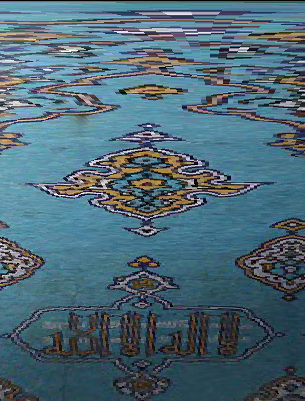
\includegraphics[height=4cm]{comparison-1}\label{compInputs:f1}}
	\qquad
	\subfloat[]{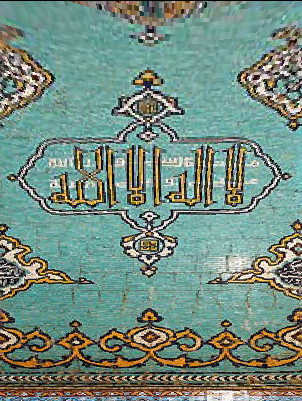
\includegraphics[height=4cm]{comparison-2}\label{compInputs:f2}}
	\caption{قطاع‌های استفاده‌شده برای مقایسه}
	\label{compInputs}
\end{figure}


\subsection{ادغام تصاویر در فضای گرادیان} \label{imageFusion}
در این قسمت از 
\lr{Multi-exposure and multi-focus image fusion in gradient domain\cite{paul2016multi}}
برای تولید بافت استفاده شد. این الگوریتم با هدف گسترش تصویر پیاده‌سازی‌ نشده و برای ادغام تصاویر یک صحنه استفاده می‌شود. برای اجرای این الگوریتم متناسب با هدف ما، باید ورودی‌ها را به فرمت مناسبی آماده می‌کردیم. تصاویر ورودی به تعداد مناسب تکرار الگو ساخته شد و هر قطاع در یک تصویر جدا قرار گرفت. ورودی‌های تولید‌شده از قطاع از لحاظ افقی با قطاع تصویر قبلی و بعدی خود تعداد شش پیکسل \gls{Overlap} دارد که برای اجرای الگوریتم نیاز بوده است. وجود ناحیه‌های هم‌پوشانی بین تصاویر ورودی قطاع برای اجرای درست الگوریتم الزامی است. بعد از به دست آوردن خروجی از الگوریتم، قسمت هم‌پوشانی تیره‌تر از نواحی دیگر بافت خواهد بود. این قسمت‌ها در انتها حذف می‌شود تا بافت نهایی تولید شود.

نمونه‌ی ورودی مناسب برای اجرای الگوریتم با سه قطاع در شکل \ref{properInputs1} آمده است. حاشیه‌های دور تصاویر برای نمایش مناسب رنگ سفید قرار داده شده است و جزو تصاویر نیستند. هر تصویر در نواحی دیگر به جز قطاع، یک رنگ ثابت خواهد بود. این رنگ می‌تواند سفید، خاکستری (دقیقا میانه‌ی سفید و سیاه) و سیاه باشد. نتایج نشان داد استفاده از رنگ سفید بهترین نتیجه را داشت.
\setlength{\fboxsep}{0pt}%
\begin{figure}[h!]
	\centering
	\subfloat[]{\fbox{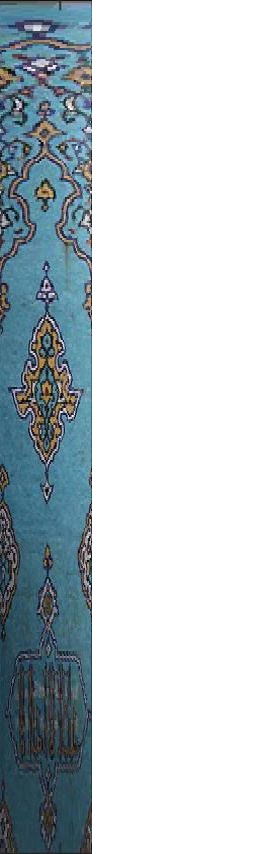
\includegraphics[height=4cm]{comparison-3}\label{properInputs1:f1}}}
	\qquad
	\subfloat[]{\fbox{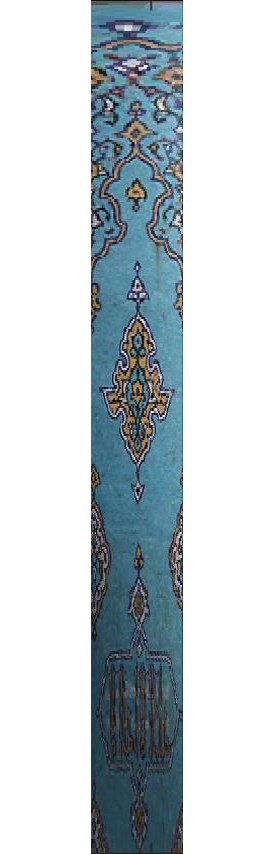
\includegraphics[height=4cm]{comparison-4}\label{properInputs1:f2}}}
	\qquad
	\subfloat[]{\fbox{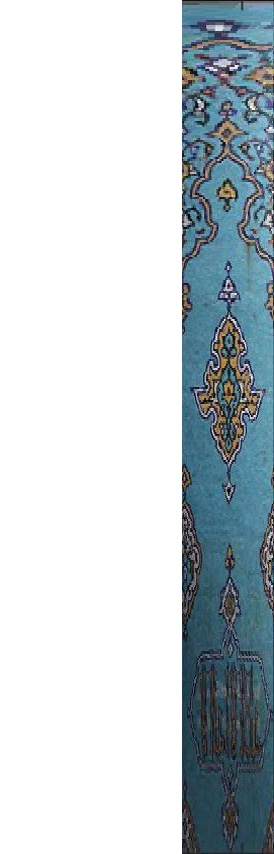
\includegraphics[height=4cm]{comparison-5}\label{properInputs1:f3}}}
	\caption{ورودی‌های مناسب برای الگوریتم ادغام تصاویر در فضای گرادیان}
	\label{properInputs1}
\end{figure}

 در شکل \ref{grayResult} نتایج تولید شده با استفاده از رنگ خاکستری برای نواحی غیر قطاع نمایش داده شده است. می‌توان از این خروجی نتیجه گرفت که چون رنگ خاکستری آنقدر متفاوت با رنگ خود قطاع نبوده است، الگوریتم تغییر مناسبی در رنگ و شدت نور قطاع ایجاد نکرده و شدت نور و رنگ در طول قطاع به ظاهر مناسبی دست پیدا نکرده است. این نتیجه هر چه از رنگ سفید دور می‌شویم، بیشتر مشاهده می‌شود. در نتیجه برای تولید نتایج مناسب با استفاده از این روش، از رنگ سفید برای نواحی غیرقطاع ورودی استفاده شده است. 
\begin{figure}[h!]
	\centering
	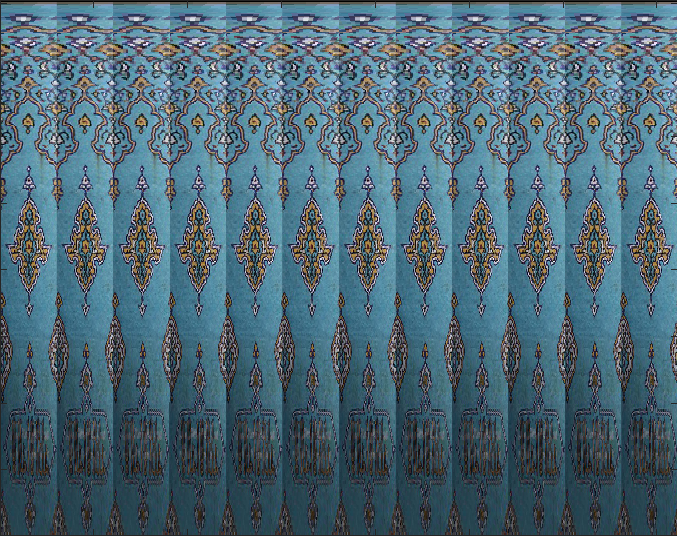
\includegraphics[height=5cm]{comparison-6}
	\caption{خروجی الگوریتم ادغام تصاویر با استفاده از رنگ خاکستری برای نواحی قیر غطاع}
	\label{grayResult}
\end{figure}

در ابتدا با استفاده از ورودی‌های مشابه با قالب شکل \ref{properInputs1}، ورودی‌ها را برای دوازده تکرار قطاع آماده کردیم و این تصاویر را به الگوریتم دادیم تا نتایج را تولید کنیم. نتایج تولید شده در شکل \ref{twelveRep} آمده است. مشخص است الگوریتم در یکسان‌سازی شدت نور عملکرد مناسبی داشته و برای یکسان‌سازی رنگ قطاع، آن را روشن‌تر کرده است که با این کار شرایط نوری در طول قطاع به طور مناسبی هموار شده است. مشکلی که در نتیجه مشاهده می‌شود، انتشار رنگ سفید در بعضی نواحی است. به طور مثال در امتداد خطی که از مرکز قطاع‌ها می‌گذرد، می‌توان مشاهده کرد رنگ سفید از چپ قطاع به سمت مرکز انتشار یافته و حاشیه‌ی قطاع‌ها را مشخص کرده است. در این حالت، اولین کاری که به نظر راه‌حل این مشکل است، تغییر رنگ سفید به رنگی نزدیک‌تر به رنگ خود قطاع‌ها می‌باشد. با انجام اینکار ما به نتیجه‌ی شکل \ref{grayResult} دست پیدا کردیم که ویژگی‌هایش را شرح دادیم.
\begin{figure}[h!]
	\centering
	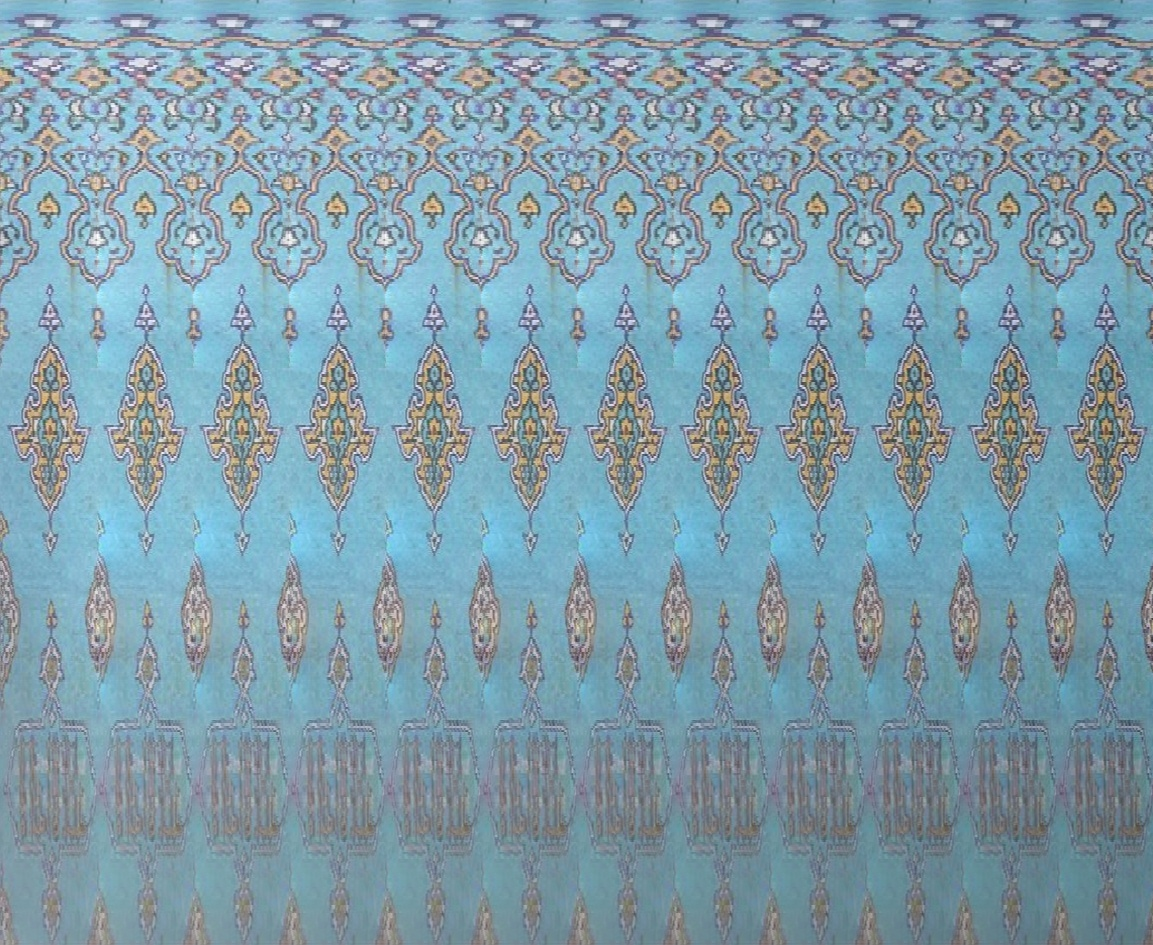
\includegraphics[height=5cm]{comparison-7}
	\caption{خروجی الگوریتم ادغام تصاویر با دوازده تکرار قطاع}
	\label{twelveRep}
\end{figure}

راه‌حل بعدی که پیاده‌سازی شد، اجرای الگوریتم به صورت قدم‌به‌قدم بوده است. در این روش، هر مرحله تنها دو تصویر با هم ادغام و ورودی‌های هر مرحله، با استفاده از خروجی قدم قبلی تولید می‌شوند. خروجی مرحله قبلی یک بار از سمت چپ با رنگ سفید گسترش می‌یابد و یک بار از سمت راست تا ورودی‌های مرحله فعلی را تشکیل دهد. این روش را با سه قدم اجرا کردیم: ابتدا با ورودی‌های تولید‌شده از قطاع اولیه، سپس با ورودی‌های تولید‌شده از دو قطاع به هم چسبیده و در انتها با استفاده از ورودی‌های تولید‌شده از چهار قطاع به هم چسبیده. نتایج این روش در شکل \ref{stepByStepRes} آورده شده است. نتایج برای قدم اول (\ref{stepByStepRes:f1}) و قدم دوم (\ref{stepByStepRes:f2}) مناسب هستند و به نظر مشکل انتشار رنگ سفید را هم ندارند. اما زمانی که به قدم آخر (\ref{stepByStepRes:f3}) می‌رسیم، مشاهده می‌شود به دلیل زیاد شدن مساحت رنگ سفید و زیاد شدن فاصله‌ی منطقه‌ی هم‌پوشانی از دو طرف تصویر، الگوریتم نتوانسته نتایج خوبی داشته باشد و علاوه بر به هم خوردن رنگ کلی بافت، خط اتصال میانی نیز به وضوح مشخص است.
\begin{figure}[h!]
	\centering
	\subfloat[]{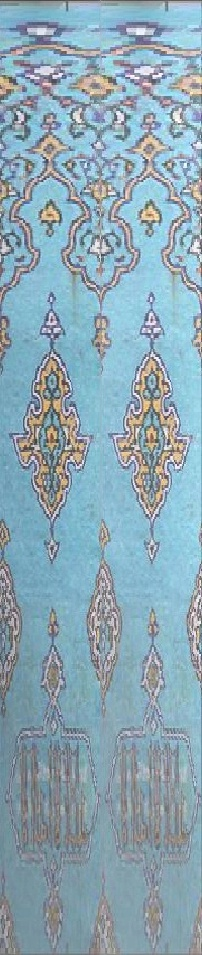
\includegraphics[height=5cm]{comparison-8}\label{stepByStepRes:f1}}
	\qquad
	\subfloat[]{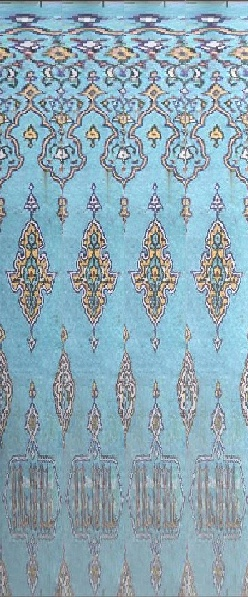
\includegraphics[height=5cm]{comparison-9}\label{stepByStepRes:f2}}
	\qquad
	\subfloat[]{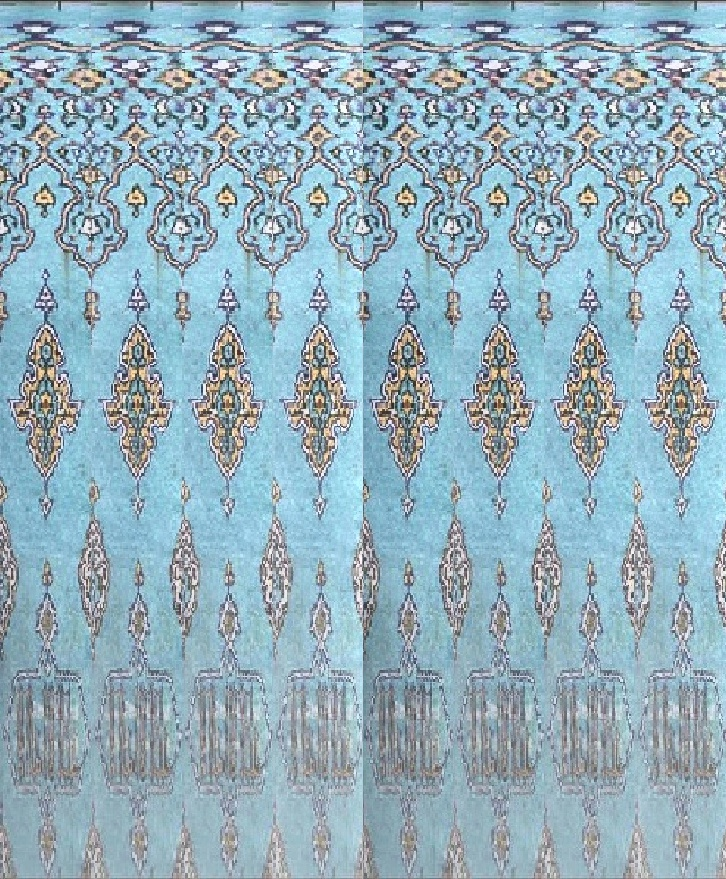
\includegraphics[height=5cm]{comparison-10}\label{stepByStepRes:f3}}
	\caption{اجرای الگوریتم ادغام تصاویر به صورت قدم‌به‌قدم}
	\label{stepByStepRes}
\end{figure}

\subsection{روش‌های یادگیری عمیق} \label{deepLearningRes}
در این قسمت با استفاده از دو روش مبتنی بر یادگیری عمیق  نتایج را تولید و تحلیل کردیم. با مشاهده نتایج، به نظر می‌رسد استفاده از یادگیری عمیق برای حفظ \gls{Structure} الگو مناسب نیست و نمی‌تواند بافت مناسب را تولید کند.

\subsubsection{تولید بافت با استفاده از شبکه عصبی پیچشی} \label{TexSynConvSec}
با استفاده از پژوهش 
\lr{Texture Synthesis Using Convolutional Neural Networks\cite{gatys2015texture}} 
نتایج این قسمت تولید شد. ورودی و خروجی الگوریتم در شکل \ref{TexSynConv} مشاهده می‌شود. در این شکل، تصویر \ref{TexSynConv:f1} ورودی الگوریتم و تصویر \ref{TexSynConv:f2} خروجی برای گسترش سه برابر عرض ورودی و طول برابر با ورودی است. خروجی به صورت کلی توانسته است رنگ بافت ورودی را حفظ کند و متوجه شده است رنگ قالب، رنگ پس‌زمینه است. مشکلی که در این روش مشاهده می‌شود، عدم حفظ ساختار الگو است که این باعث در‌هم‌ریختگی الگو در بافت نهایی شده است.
\begin{figure}[h!]
	\centering
	\subfloat[]{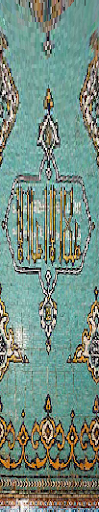
\includegraphics[height=5cm]{comparison-11}\label{TexSynConv:f1}}
	\qquad
	\subfloat[]{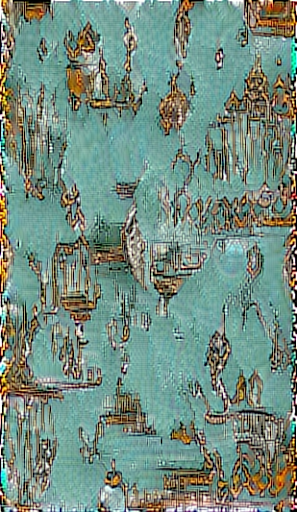
\includegraphics[height=5cm]{comparison-12}\label{TexSynConv:f2}}
	\caption{اجرای الگوریتم تولید بافت با استفاده از شبکه عصبی پیچشی}
	\label{TexSynConv}
\end{figure}

\subsubsection{بافت‌های بهینه}
این قسمت نتایج تولید شده با استفاده از الگوریتم 
\lr{Optimal Textures\cite{risser2020optimal}}
آمده است. این الگوریتم دو هدف متفاوت را می‌تواند اجرا کند. هدف اول مانند \ref{TexSynConvSec}، برای گسترش تصاویر است. در این هدف، ما برای تنظیمات الگوریتم، عرض خروجی را چهار برابر و طول آن را برابر با ورودی مشخص کردیم. ورودی و خروجی الگوریتم برای این هدف در شکل \ref{OpTex1} آمده است که تصویر \ref{OpTex1:f1} ورودی الگوریتم و تصویر \ref{OpTex1:f2} خروجی تولید‌شده را نمایش می‌دهد. خروجی این قسمت ویژگی‌های مشابه با \ref{TexSynConvSec} دارد که با توجه به عدم تمرکز بر روی مشکل حفظ ساختار الگو‌ها در این پژوهش نسبت به پژوهش قبلی، این نتایج آن چنان دور از انتظار نبود.
\begin{figure}[h!]
	\centering
	\subfloat[]{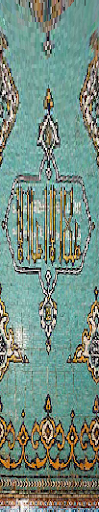
\includegraphics[height=5cm]{comparison-13}\label{OpTex1:f1}}
	\qquad
	\subfloat[]{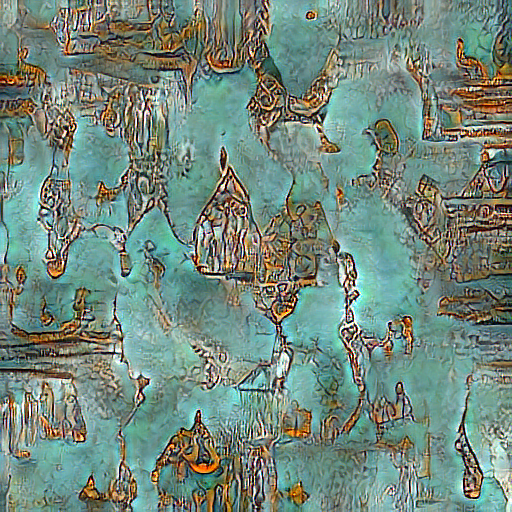
\includegraphics[height=5cm]{comparison-14}\label{OpTex1:f2}}
	\caption{اجرای الگوریتم بافت‌های بهینه با هدف گسترش}
	\label{OpTex1}
\end{figure}

هدف دیگری که پژوهش بافت‌های بهینه ارائه می‌دهد، ادغام تصاویر ‌(مانند \ref{imageFusion}) است. ورودی و خروجی اجرای الگوریتم برای این هدف در شکل \ref{OpTex2} آمده است. تصاویر \ref{OpTex2:f1} و \ref{OpTex2:f2} ورودی تولید شده برای این هدف هستند و تصویر \ref{OpTex2:f3} خروجی الگوریتم را نمایش می‌دهد. با استفاده از این هدف، نتایج باز هم مناسب نیستند و به رنگ سفید وزن بیشتری نسبت به الگوی ورودی داده شده است.
\begin{figure}[h!]
	\centering
	\subfloat[]{\fbox{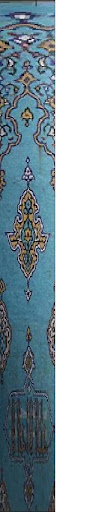
\includegraphics[height=5cm]{comparison-15}\label{OpTex2:f1}}}
	\qquad
	\subfloat[]{\fbox{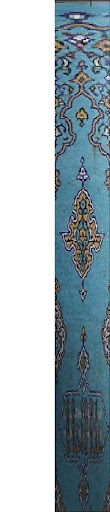
\includegraphics[height=5cm]{comparison-16}\label{OpTex2:f2}}}
	\qquad
	\subfloat[]{\fbox{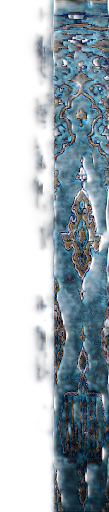
\includegraphics[height=5cm]{comparison-17}\label{OpTex2:f3}}}
	\caption{اجرای الگوریتم بافت‌های بهینه برای ادغام تصاویر}
	\label{OpTex2}
\end{figure}

\subsection{روش‌های مبتنی بر وصله} \label{patchBasedRes}
در این قسمت نتایج را با یک پیاده‌سازی روش‌های مبتنی بر وصله\cite{patchBaseGit} که با استفاده از پژوهش‌های 
\lr{Image Quilting} 
و
\lr{Real-Time Texture Synthesis by Patch-Based Sampling\cite{patchBasedSampling}} 
نوشته شده است، تولید کردیم. در ابتدا الگوریتم را با استفاده از یک قطاع به عنوان ورودی، اجرا کردیم. ورودی (قسمت سمت راست تصویر) و خروجی (قسمت سمت چپ تصویر) در شکل \ref{patch1} نمایش داده شده است. گسترش انتخاب شده برای طول و عرض دو برابری خروجی نسبت به ورودی بوده‌است. وصله‌های انتخاب شده برای تولید خروجی ساختار مناسبی ندارند و الگوریتم با استفاده از معیار فاصله خود نتوانسته وصله‌های مناسبی را انتخاب کند.
\begin{figure}[h!]
	\centering
	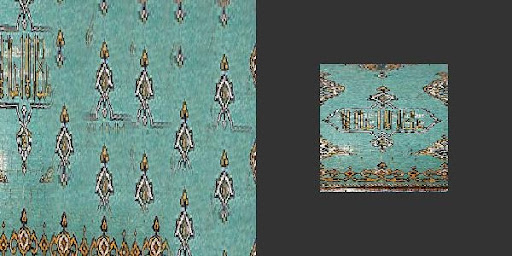
\includegraphics[height=5cm]{comparison-18}
	\caption{ورودی و خروجی روش مبتنی بر وصله با یک قطاع}
	\label{patch1}
\end{figure}
\newline
برای اینکه امکان تولید نتایج مناسب را بالا ببریم، از خروجی اتصال چهار قطاع، که با استفاده از \ref{imageFusion} تولید شده است، به عنوان ورودی برای الگوریتم انتخاب کردیم. ورودی و خروجی در شکل \ref{patch2} آمده است. با استفاده از چهار قطاع، الگوریتم توانسته با استفاده از معیار فاصله خود، وصله‌های بهتری برای خروجی پیدا کند، اما در بعضی مناطق باز هم دچار اشتباه شده و خروجی ساختار کامل را رعایت نکرده است. به نظر می‌رسد تضمین کاملی برای انتخاب وصله‌های مناسب توسط الگوریتم وجود ندارد. مشکل دیگری که پر این الگوریتم وجود دارد، انتخاب وصله‌ها به صورت مربعی است. تلاش شد با تغییر کد کاری کرد که نیازی به انتخاب فرمت مربعی برای خروجی و وصله‌ها نباشد، اما به نتیجه نرسید و اندازه‌ها با یکدیگر هماهنگ نشدند. دلیل اصلی این اتفاق تفاوت ترتیب طول و عرض در ماتریس تصاویر 
\lr{OpenCV} 
و 
 \lr{NumPy}
 بود که به علت مربعی بودن پیاده‌سازی اصلی، در خیلی از قسمت‌های کد این اشتباه رخ داده و امکان تغییر نبود.
\begin{figure}[h!]
	\centering
	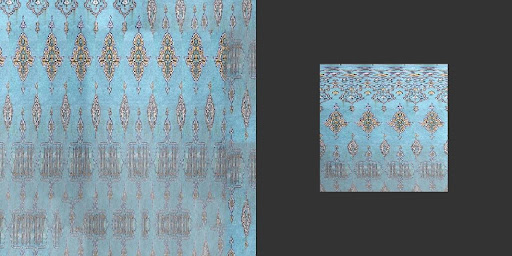
\includegraphics[height=5cm]{comparison-19}
	\caption{ورودی و خروجی روش مبتنی بر وصله با چهار قطاع}
	\label{patch2}
\end{figure}

\subsection{آینده کردن تصویر} \label{mirroringRes}
در این قسمت با استفاده از روش آینه‌کردن تلاش می‌شود تصویر از لحاظ رنگی و شدت نوری هموار شود. در صورتی که قطاع در نظر گرفته‌شده حاوی طرح متقارن باشد، استفاده از این تکنیک هم در فضای RGB و هم در فضای LUV می‌تواند هموار کردن را به صورت مناسبی انجام دهد. مشکل اصلی این الگوریتم در شکل \ref{mirroring} نمایش داده شده است. این خروجی برای قطاع \ref{compInputs:f1} تولید شده است که حاوی قسمت متنی بوده است. خروجی این روش، با اینکه از لحاظ نوری و رنگی هموار است و در مکان‌های اتصال قطاع‌ها خطی مشاهده نمی‌شود، قسمت متنی قطاع را به هم ریخته و ساختار را خراب کرده است.
\begin{figure}[h!]
	\centering
	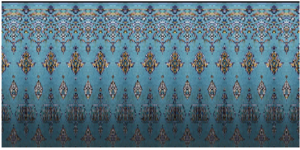
\includegraphics[height=5cm]{comparison-20}
	\caption{خروجی استفاده از روش آینه‌کردن در قطاع حاوی متن}
	\label{mirroring}
\end{figure}

\subsection{الگوریتم ارائه‌شده} \label{ourAlgCompRes}
در این قسمت نتایج تولید شده با استفاده از روش ما با استفاده از ورودی‌های \ref{compInputs} تولید شده است. در شکل \ref{compOurs1} بافت تولید شده برای ورودی قطاع \ref{compInputs:f1} آمده است. همانطور که در تصویر مشخص است، الگوریتم ما توانسته به صورت مناسب مرز‌های بین قطاع‌ها را حذف کند و بافت همواری را تولید کند. در خروجی مشخص است که مشکل انتشار رنگ سفید (مشکل مشاهده شده در بخش \ref{imageFusion}) حل شده و الگوریتم توانسته ساختار ورودی را، برخلاف روش‌های یادگیری عمیق اجرا‌شده در بخش \ref{deepLearningRes} و \ref{patchBasedRes}، حفظ کند. نسبت به روش آینه‌کردن تصاویر (بخش \ref{mirroringRes})، الگوریتم ما در هموار کردن با آن برابری می‌کند، اما مشکل در هم ریختگی قسمت متنی را ندارد.

 تنها مشکلی که در این خروجی مشاهده می‌شود، در بالای بافت تولید شده است که به صورت کامل خط بین قطاع‌ها برطرف نشده است. دلیل وجود این مشکل تفاوت زیاد نوری این بخش از قطاع در دو طرف تصویر است که به علت ساختار هندسه‌ی شیء انتخاب‌شده برای مدل‌سازی بوجود آمده. مدل انتخاب شده یک گنبد بوده که به علت هندسه‌ی آن، بخش بالای تصویر در اصل مساحت بسیار کمتری را نسبت به قسمت میانی تصویر بر روی گنبد شامل می‌شود. البته با توجه به هندسه‌ی مدل سه‌بعدی که باید بافت بر روی آن نگاشت شود، این مشکل به علت فشرده شدن بخش بالای تصویر، دیده نمی‌شود.
\begin{figure}[h!]
	\centering
	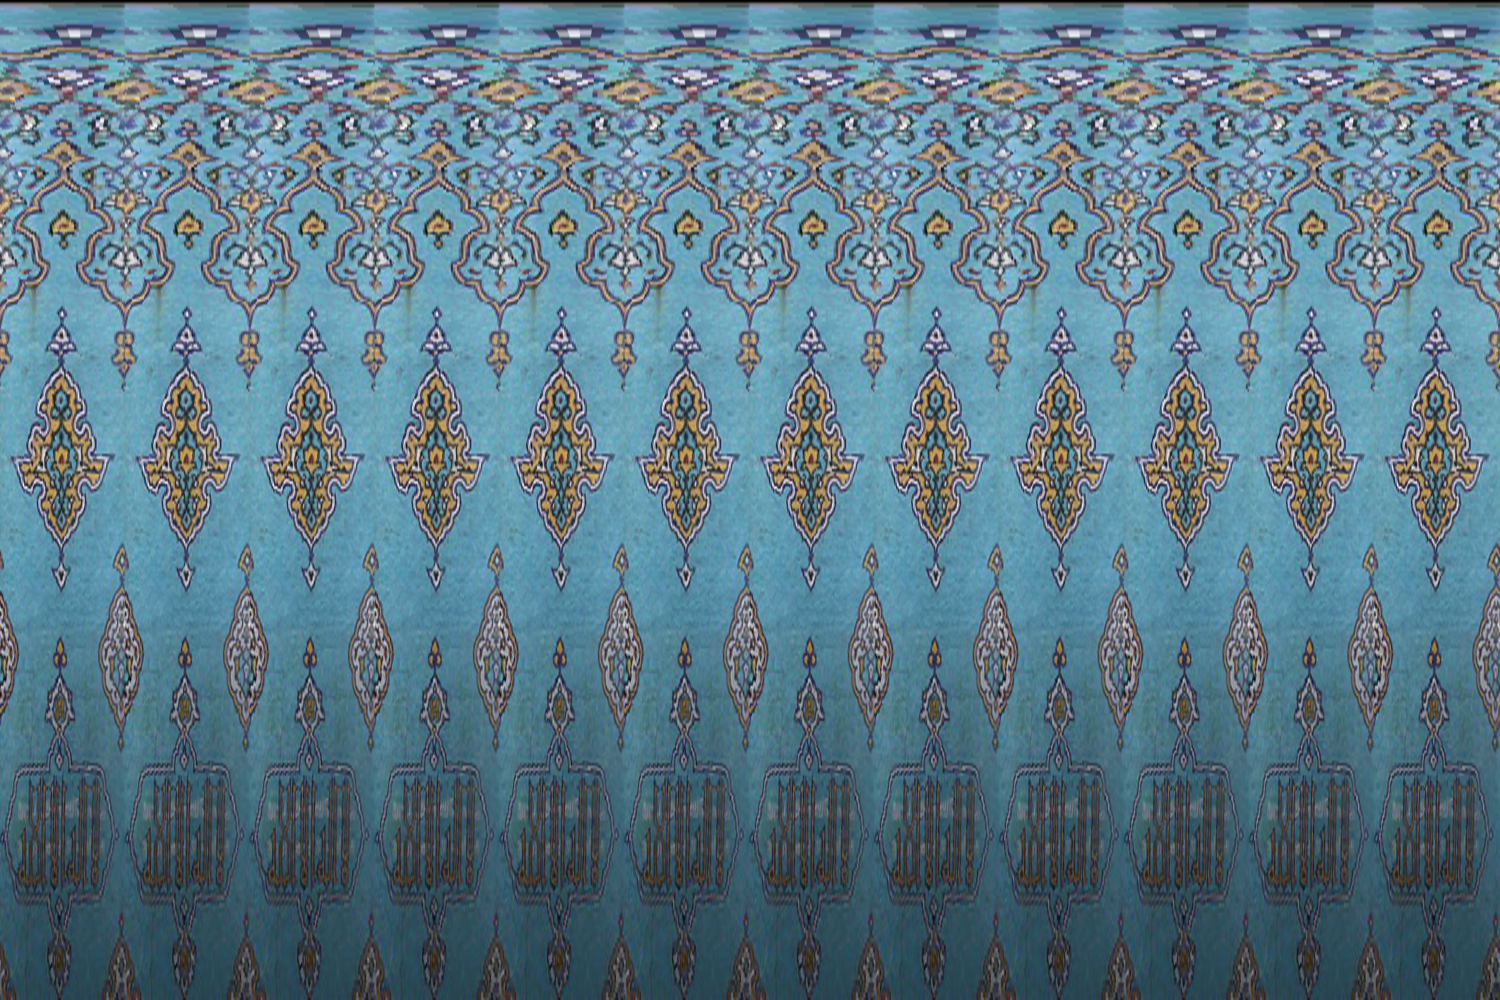
\includegraphics[height=5cm]{comparison-21}
	\caption{بافت تولید شده از الگوریتم ارائه‌شده برای ورودی \ref{compInputs:f1}}
	\label{compOurs1}
\end{figure}

در شکل \ref{compOurs2} بافت تولید شده برای قطاع \ref{compInputs:f2} نمایش داده شده است. همانطور که مشخص است، این بافت مشکلات خروجی‌های بخش‌های قبلی را ندارد و از لحاظ رنگی و نوری هموار می‌باشد. ایرادی که امکان دارد از این بافت گرفته شود، وجود انعکاس نور در وسط و پایین تصویر است که  همراه با قطاع بوده و در هر تکرار قطاع دیده می‌شود. با توجه به اینکه در روش ارائه‌شده، ما تمرکز خود را بر روی نواحی حاشیه قطاع قرار داده‌ایم، وجود اعوجاج در میانه‌ی قطاع برای ما اهمیتی ندارد و آن را بررسی نمی‌کنیم. در نتیجه انتخاب قطاع مناسب برای تولید بافت بدون مشکل در الگوریتم ما مهم است.
\begin{figure}[h!]
	\centering
	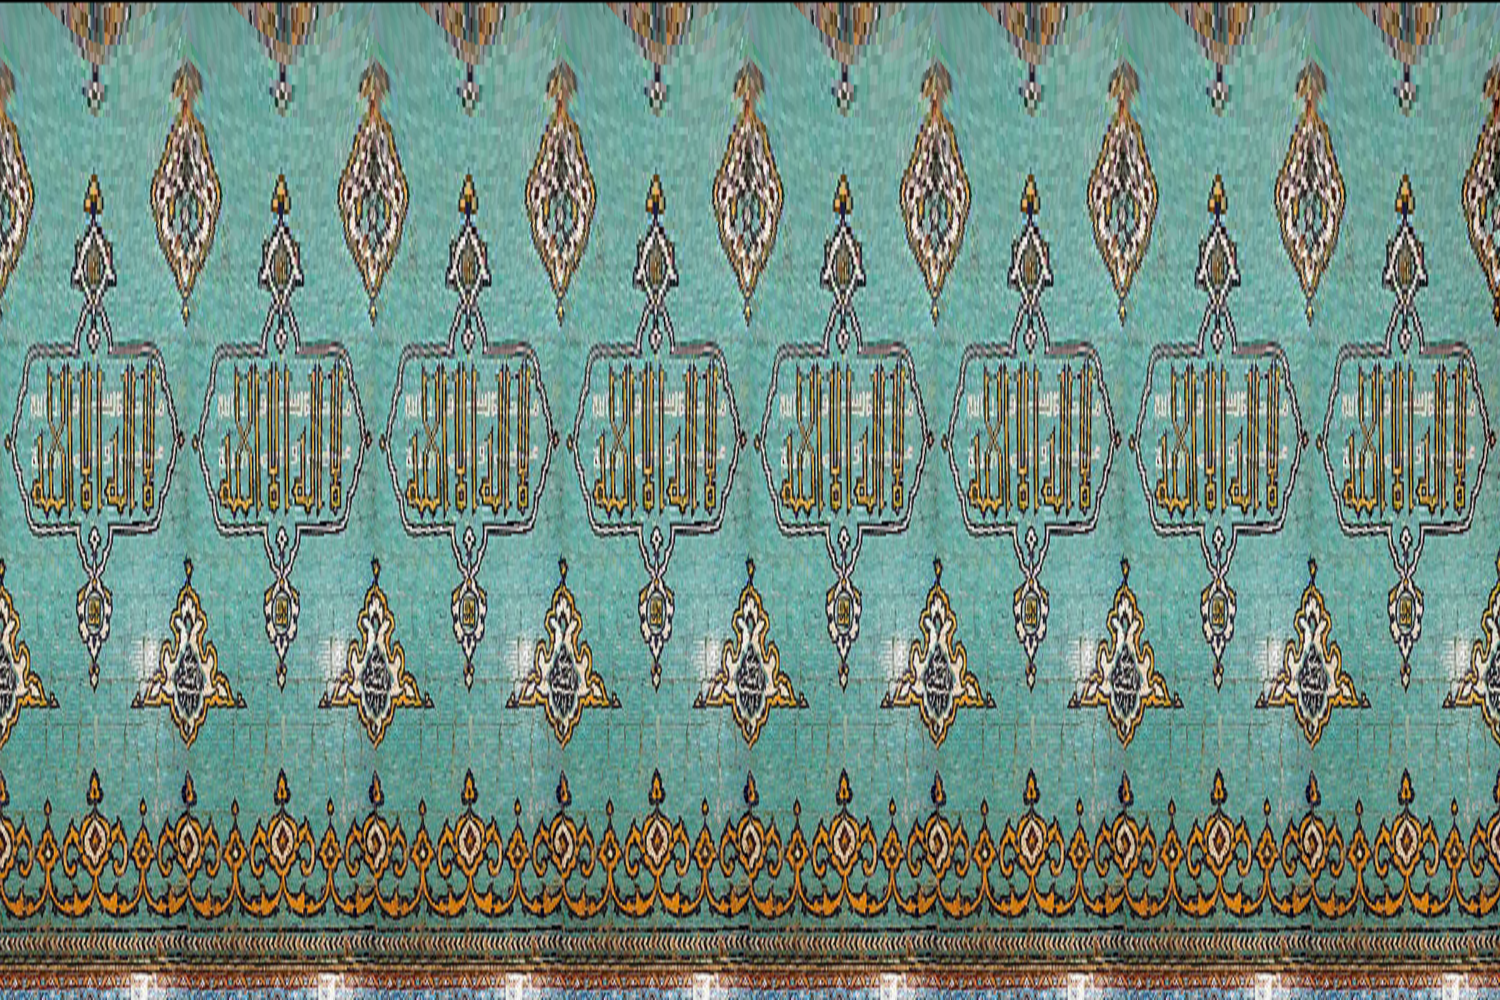
\includegraphics[height=5cm]{comparison-22}
	\caption{بافت تولید شده از الگوریتم ارائه‌شده برای ورودی \ref{compInputs:f2}}
	\label{compOurs2}
\end{figure}

\section{بازسازی سه‌بعدی با استفاده از یک تصویر}
در این قسمت نتایج استفاده از روش ارائه‌شده در مسئله‌ی تولید بافت برای بازسازی سه‌بعدی از یک تصویر را نمایش داده‌ایم. برای مدل‌سازی هندسه و استخراج بافت رویی شیء، از الگوریتم رویه دورانی استفاده شده است. روش استفاده شده در آن الگوریتم، به صورت پیش‌فرض، تکرار الگوی رویی برای قسمت پشتی شیء بوده که ما این روش را برای بعضی از اشیاء اجرا و نتایج آن را با نتایج تولید‌شده با استفاده از روش خودمان مقایسه کردیم.

در ابتدا برای تکمیل کردن نتایج بخش قبل، در شکل \ref{res1In} تصویر اصلی شیء که قطاع \ref{compInputs:f1} از آن استخراج شده بود، در کنار خود قطاع آورده شده است. همانطور که گفته‌شد، هندسه‌ی مدل به صورت جداگانه از تصویر \ref{res1In:f1} استخراج می‌شود و تمرکز ما تنها بر روی تولید بافت بوده است.
\begin{figure}[h!]
	\centering
	\subfloat[تصویر اصلی شیء]{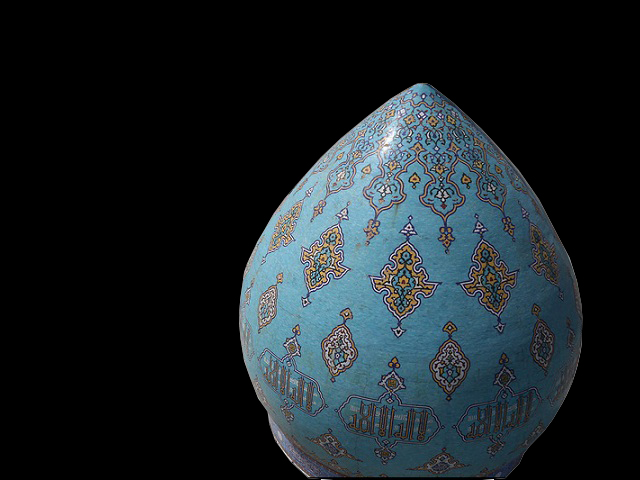
\includegraphics[height=4cm]{ourRes-1}\label{res1In:f1}}
	\qquad
	\subfloat[قطاع استخراج‌شده]{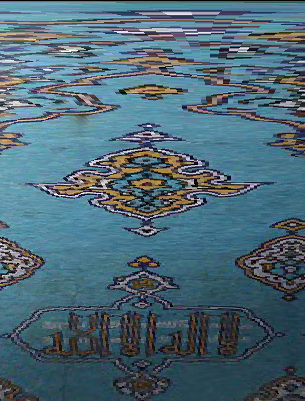
\includegraphics[height=4cm]{ourRes-2}\label{res1In:f2}}
	\caption{ورودی‌های اول الگوریتم ارائه‌شده}
	\label{res1In}
\end{figure}
\newline
بافت تولید‌شده با استفاده از روش ارائه‌شده در شکل \ref{res1Out} آورده شده است که ویژگی‌های آن در بخش \ref{ourAlgCompRes} شرح داده شد. این خروجی با دوازده تکرار قطاع مشخص‌شده در \ref{res1In:f2} تولید شده است.
\begin{figure}[h!]
	\centering
	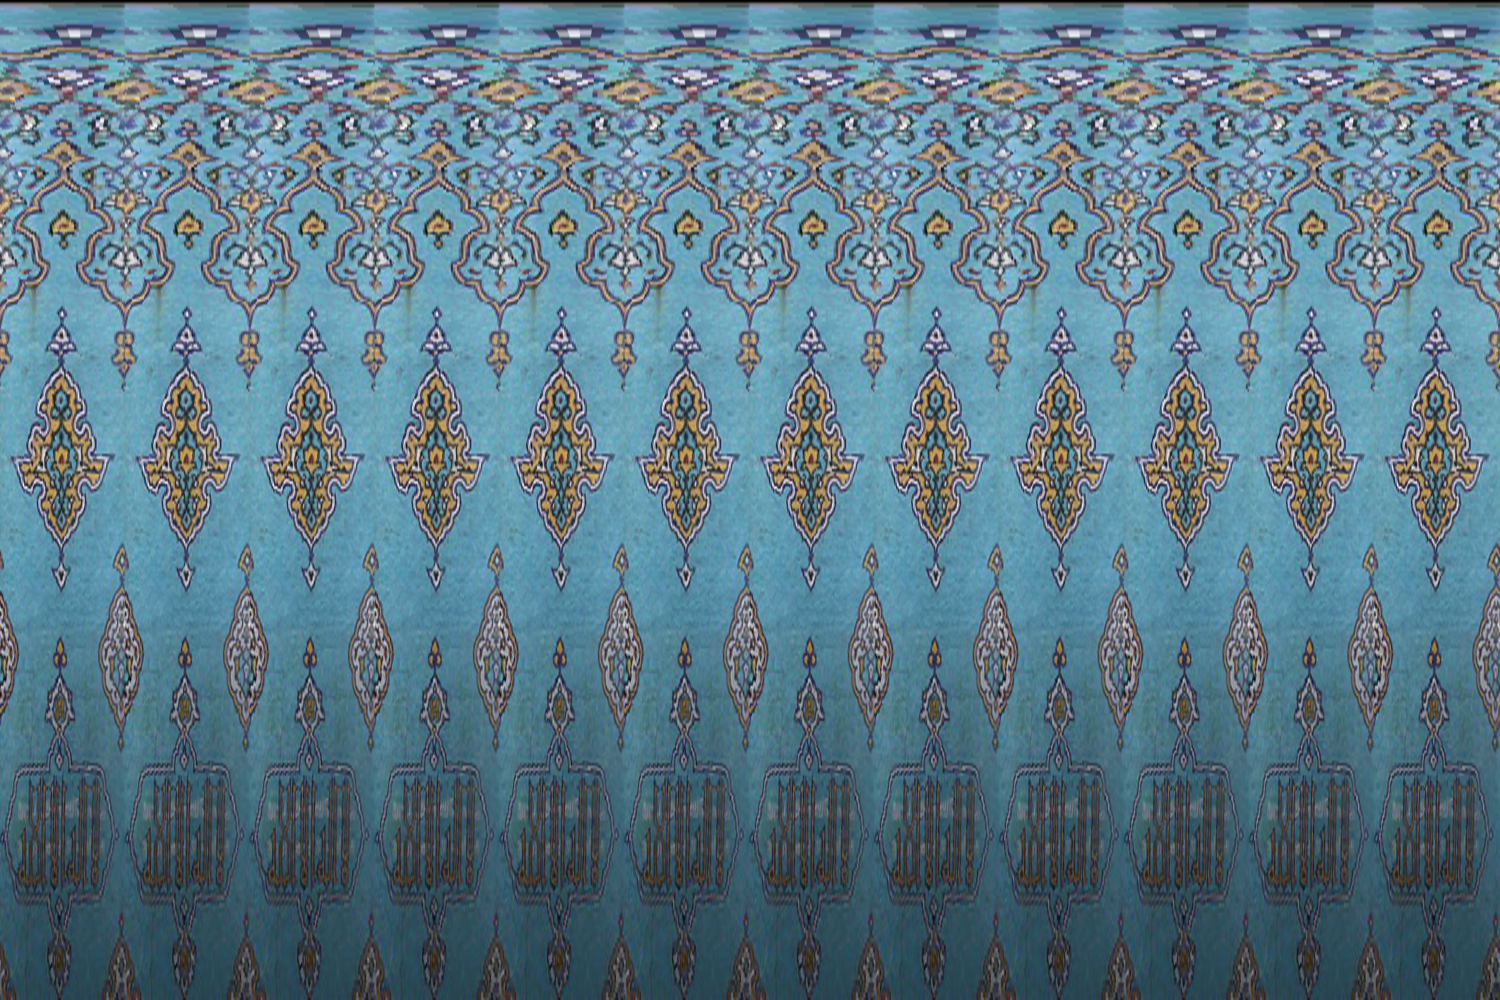
\includegraphics[height=5cm]{ourRes-3}
	\caption{بافت تولید شده از الگوریتم ارائه‌شده برای ورودی اول}
	\label{res1Out}
\end{figure}
\newline
خروجی تولید‌شده پس از نگاشت بافت خروجی از روش ما بر روی هندسه‌ی تولید‌شده، در شکل \ref{res1_3DOut} آورده شده است. بازسازی صورت گرفته از لحاظ ویژگی‌های ظاهری مناسب می‌باشد. هندسه سه‌بعدی استخراج‌شده ارتفاع کامل گنبد را شامل نشده اما بافت استخراج شده نیز همین ویژگی را دارد. تنها مشکلی که به ظاهر وجود دارد، یکسان نبودن تعداد تکرار قطاع در بافت تولید‌شده نسبت به تصویر جسم است، که این تعداد تکرار از الگوریتم رویه دورانی استخراج شده بود. البته این مشکل را به راحتی می‌توان با انتخاب تعداد مناسب تکرار به عنوان ورودی برای الگوریتم ارائه شده حل کرد.
\begin{figure}[h!]
	\centering
	\subfloat[]{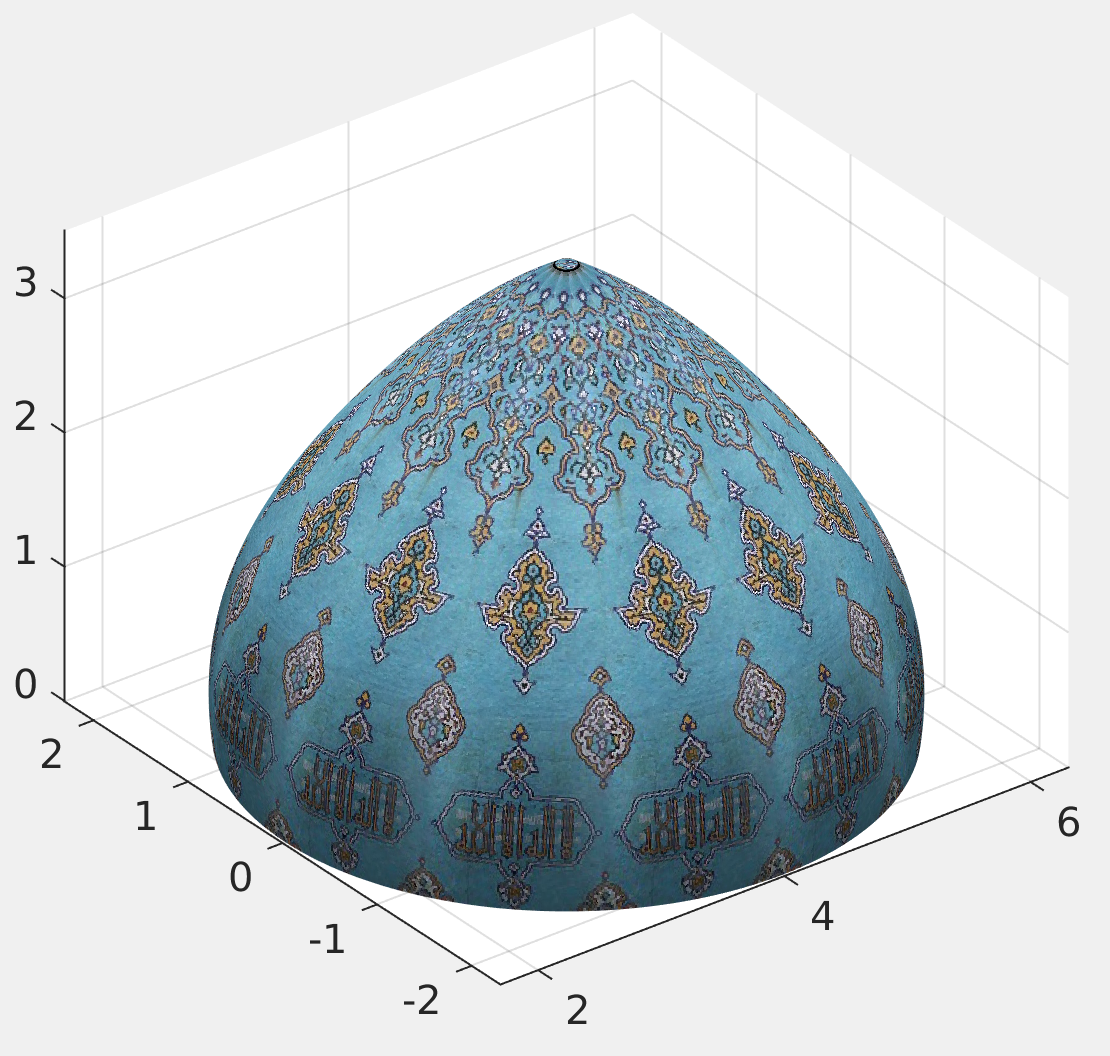
\includegraphics[height=4cm]{ourRes-4}\label{res1_3DOut:f1}}
	\qquad
	\subfloat[]{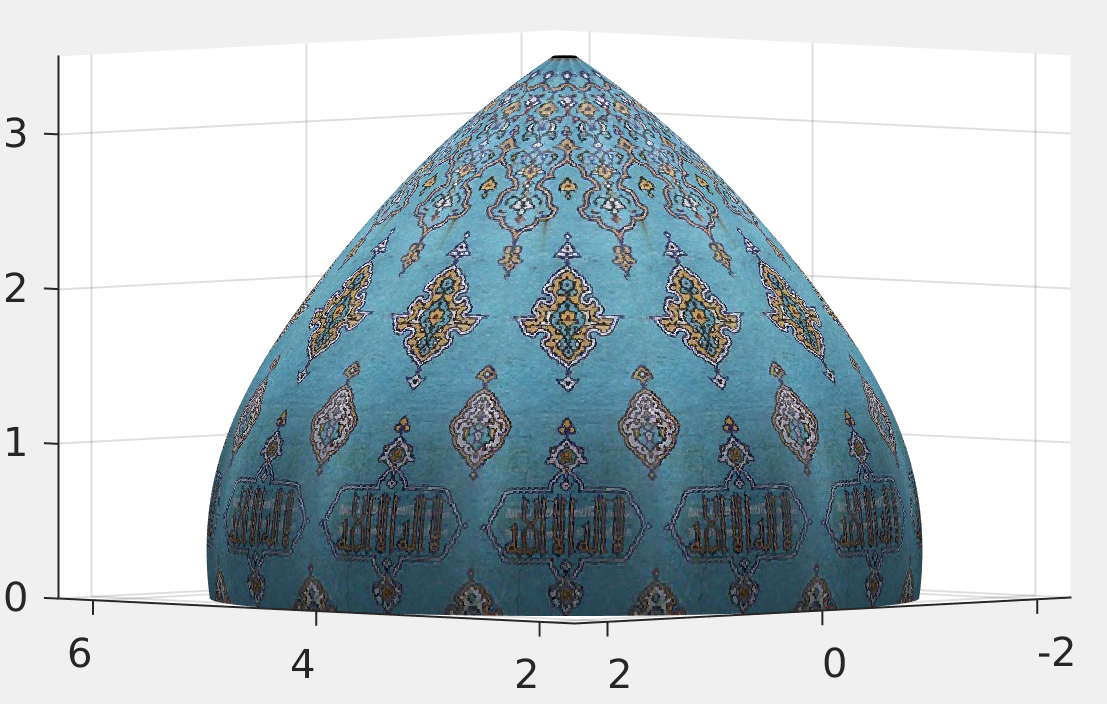
\includegraphics[height=4cm]{ourRes-5}\label{res1_3DOut:f2}}
	\caption{مدل سه‌بعدی بازسازی شده اول}
	\label{res1_3DOut}
\end{figure}

ورودی بعدی انتخاب‌شده در شکل \ref{res2In} آمده است که همان قطاع \ref{compInputs:f2} به همراه تصویر اصلی شیء است که قطاع از آن استخراج شده بود.
\begin{figure}[h!]
	\centering
	\subfloat[تصویر اصلی شیء]{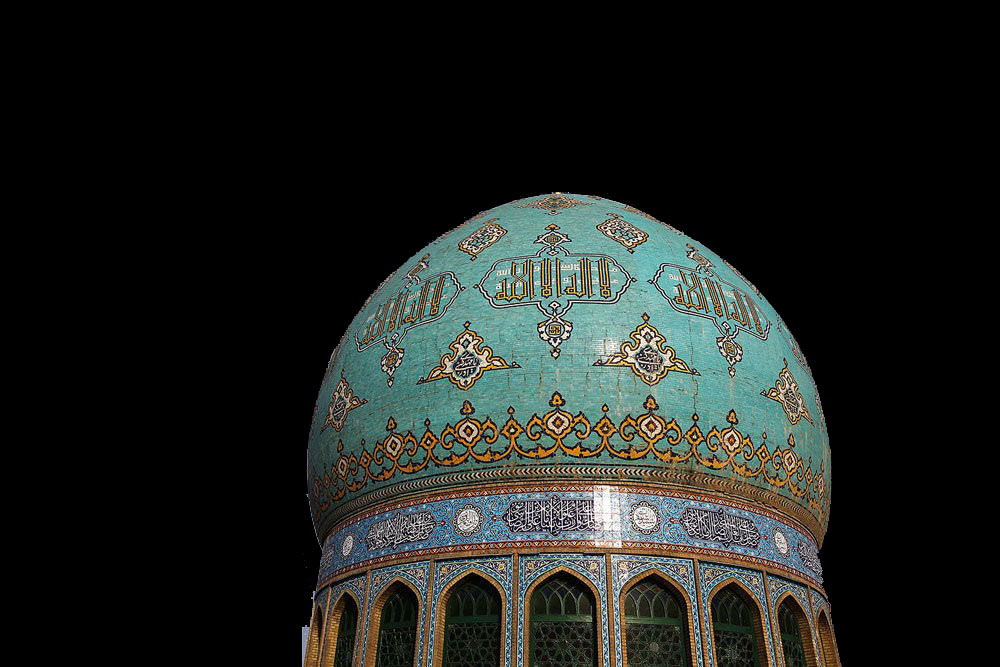
\includegraphics[height=4cm]{ourRes-6}\label{res2In:f1}}
	\qquad
	\subfloat[قطاع استخراج‌شده]{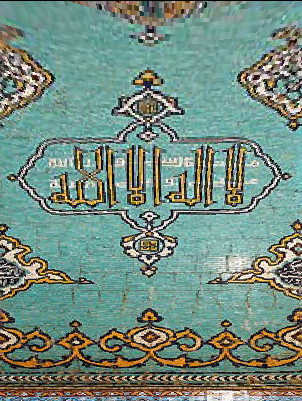
\includegraphics[height=4cm]{ourRes-7}\label{res2In:f2}}
	\caption{ورودی‌های دوم الگوریتم ارائه‌شده}
	\label{res2In}
\end{figure}
\newline
بافت تولید‌شده در شکل \ref{res2Out} آمده است که در بخش \ref{ourAlgCompRes} ویژگی‌های این بافت را نیز شرح دادیم. این بافت با هشت تکرار قطاع تولید‌شده است.
\begin{figure}[h!]
	\centering
	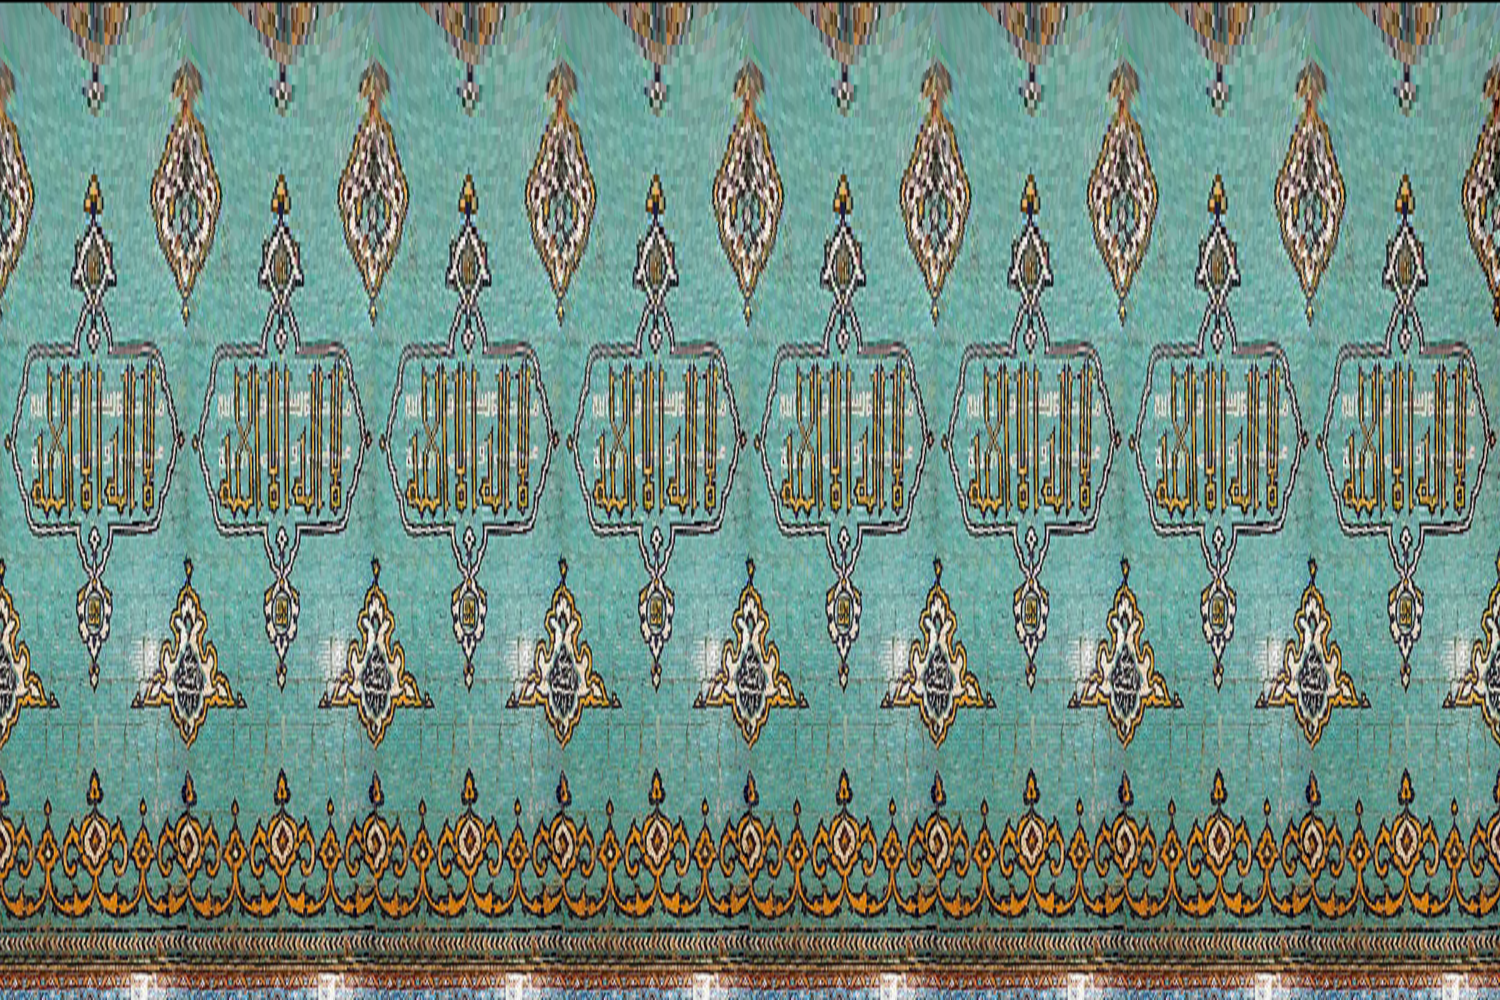
\includegraphics[height=5cm]{ourRes-8}
	\caption{بافت تولید شده از الگوریتم ارائه‌شده برای ورودی دوم}
	\label{res2Out}
\end{figure}

مدل نهایی بازسازی شده در شکل \ref{res2_3DOut} آمده است. برای این شیء هم مدل سه‌بعدی بازسازی شده کامل نیست اما الگوی متناسب استخراج شده بوده و بافت نهایی تولید‌شده هموار و مناسب است. در این شیء تکرار قطاع مناسب است و مدل سه‌بعدی نهایی شباهت مطلوبی با شیء اصلی در تصویر ورودی دارد. تنها مشکلی که در بافت مشاهده می‌شود، قسمت بالایی بافت است که به علت زاویه دوربین، از ناحیه‌ای استخراج شده که بعد از گسترش به الگوی مستطیلی، کشیدگی زیادی داشته و اندکی محو شده است. اما این مشکل به علت زاویه دوربین در تصویر ورودی بوده و روش ارائه‌شده‌ی ما بر روی این موضوع تمرکزی ندارد.
\begin{figure}[h!]
	\centering
	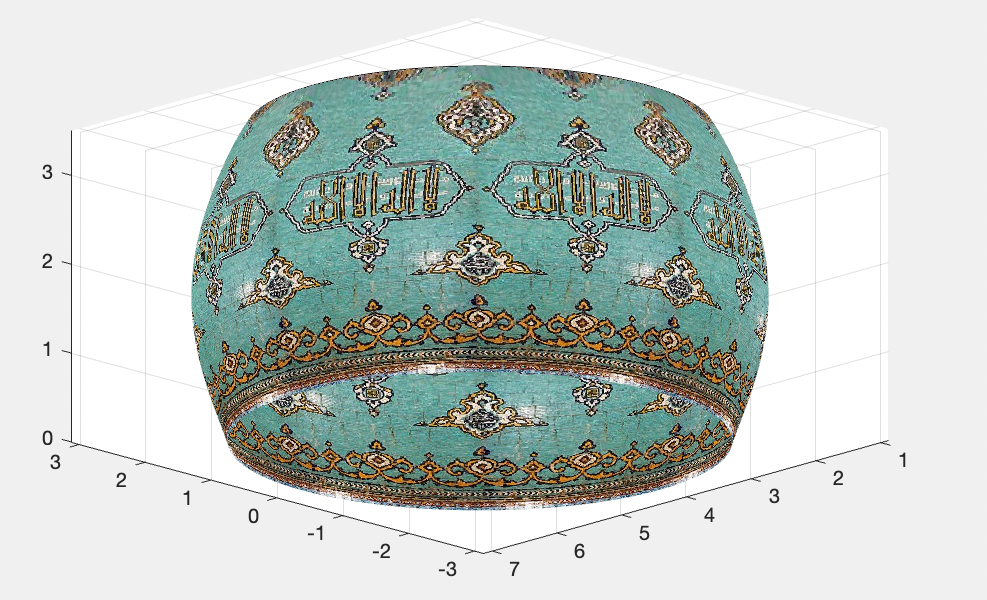
\includegraphics[height=5cm]{ourRes-9}
	\caption{مدل سه‌بعدی بازسازی شده دوم}
	\label{res2_3DOut}
\end{figure}

ورودی سوم در شکل \ref{res3In} آمده است. شیء مورد نظر (تصویر \ref{res3In:f1}) یک کوزه است که قطاع آن سه بار تکرار شده است. همانطور که از تصویر مشخص است، در صورتی که الگوی رویی شیء را برای قسمت پشت آن تکرار کنیم، در جلو و پشت شیء یک تکرار کامل قطاع داریم و در دو طرف شی هر کدام یک قسمت کوچک از قطاع وجود داردک ه تشکیل یک قطاع کامل را نمی‌دهند. مدل سه‌بعدی بازسازی‌شده با استفاده از این روش در شکل \ref{res3_bad} آمده است که این مشکل در تکرار ساده نشان می‌دهد. در تصویر \ref{res3In:f2} قطاع نهایی پس از استخراج الگو و برش آن آمده است. مشکلی که در قطاع دیده می‌شود، عمودی نبودن خط‌های دهانه‌ی کوزه است. این مشکل به علت استخراج نامناسب الگوی رویی  به دلیل دقیق نشدن هندسه‌ی مدل بر روی تصویر، پیش آمده است. با توجه به اینکه این مرحله توسط الگوریتم ارائه‌شده انجام نمی‌شود، برای بهبود این قسمت کاری انجام نشده است.
\begin{figure}[h!]
	\centering
	\subfloat[تصویر اصلی شیء]{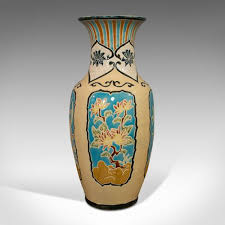
\includegraphics[height=4cm]{ourRes-11}\label{res3In:f1}}
	\qquad
	\subfloat[قطاع استخراج‌شده]{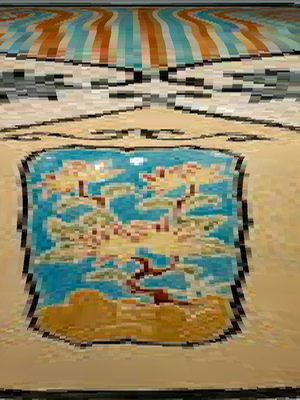
\includegraphics[height=4cm]{ourRes-12}\label{res3In:f2}}
	\caption{ورودی‌های سوم الگوریتم ارائه‌شده}
	\label{res3In}
\end{figure}
\begin{figure}[h!]
	\centering
	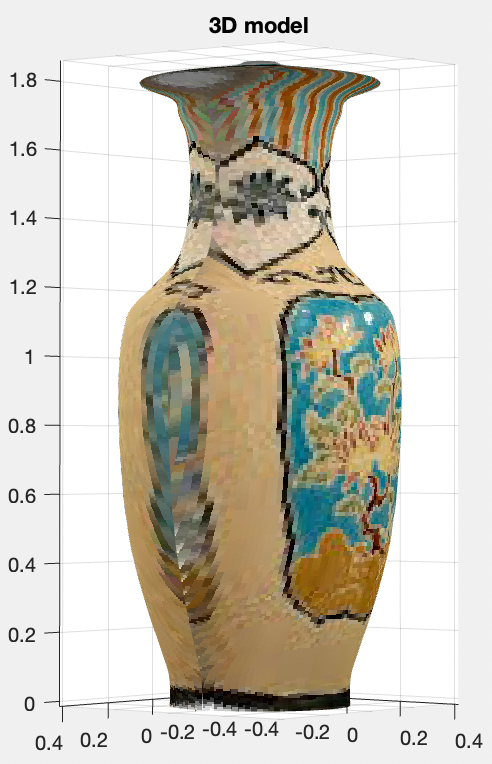
\includegraphics[height=5cm]{ourRes-10}
	\caption{مدل سه‌بعدی بازسازی‌شده برای ورودی سوم با استفاده از تکرار ساده طرح رویی برای پشت}
	\label{res3_bad}
\end{figure}

مطابق شکل \ref{res3Out}، بافت نهایی از قطاع با انجام سه تکرار تولید شده است. قطاع نهایی (\ref{res3in:f2}) با استفاده از روش رفع واپیچش، هموار‌تر شده تا در دو طرف قطاع مشکلی برای اتصال مناسب الگو‌ها به هم نداشته باشیم. بافت نهایی تولید شده به علت کم بودن کیفیت تصویر و نامنظم بودن الگوی کوزه، اندکی از لحاظ ظاهری مشکل دارد. البته این مشکل بعد از نگاشت بافت به هندسه‌ی سه‌بعدی کم‌رنگ‌تر شده است. در بافت نهایی نیز مشکل خطوط عمودی بالای الگو دیده می‌شود اما الگوریتم تلاش کرده این قسمت را هم هموار کند که مشاهده می‌شود خط محکمی در این قسمت نیز دیده نمی‌شود.
\begin{figure}[h!]
	\centering
	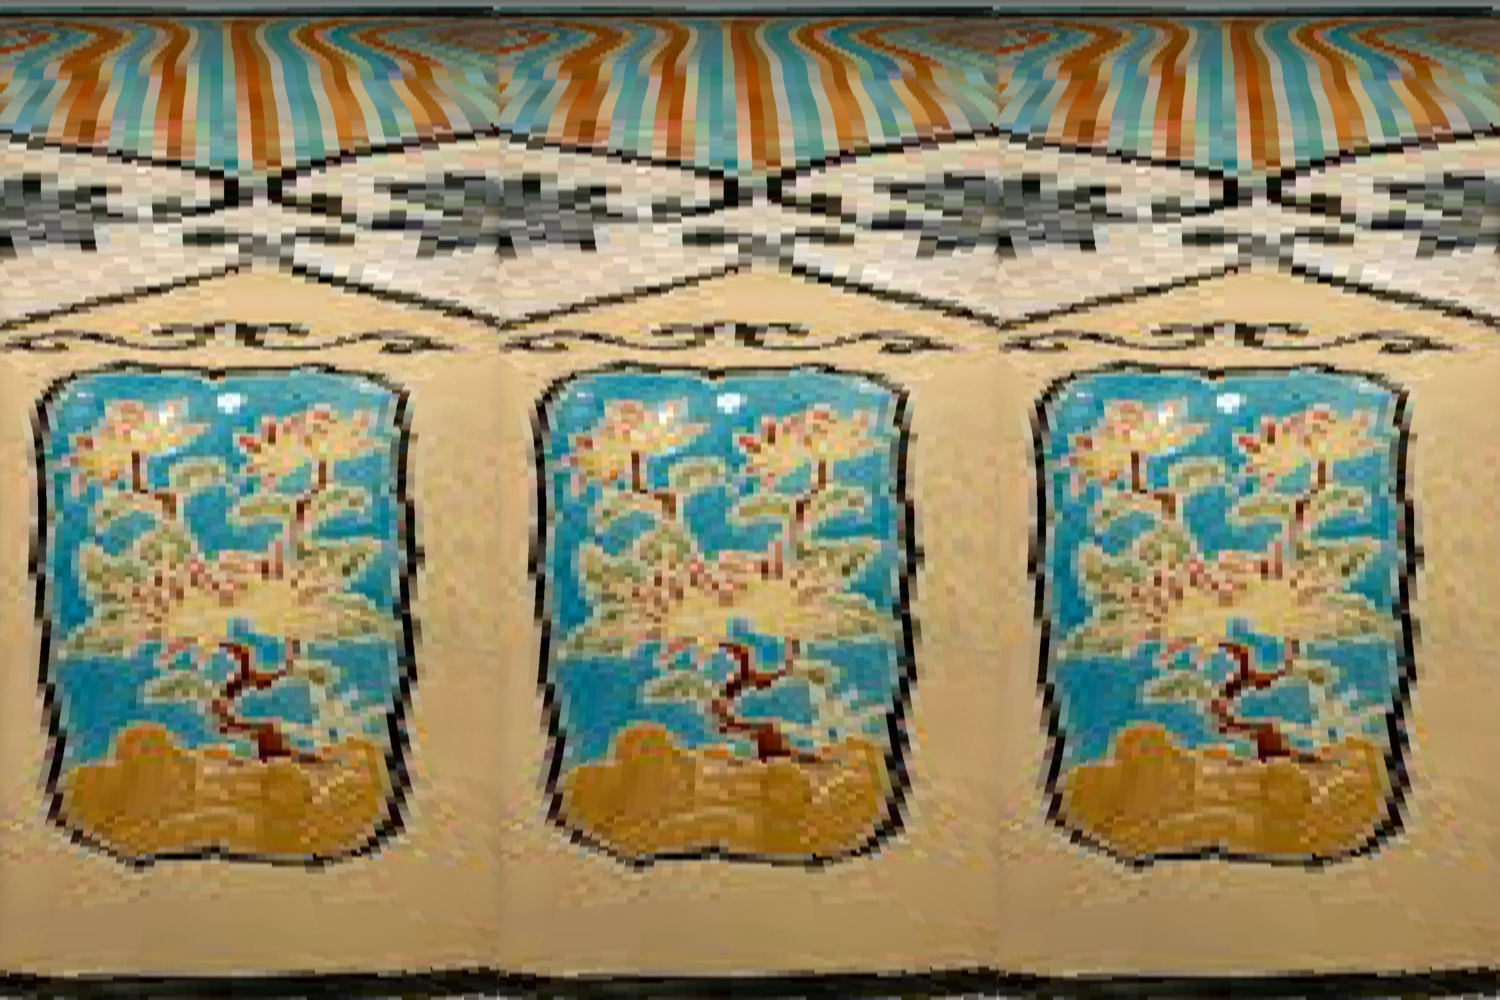
\includegraphics[height=5cm]{ourRes-13}
	\caption{بافت تولید شده از الگوریتم ارائه‌شده برای ورودی سوم}
	\label{res3Out}
\end{figure}

در شکل \ref{res3_3DOut} مدل سه‌بعدی نهایی بعد از نگاشت بافت تولید‌شده بر روی هندسه‌ی مدل آمده است. در مقایسه با شکل \ref{res3_bad}، مشاهده می‌شود روش ارائه‌شده، نتیجه‌ی مطلوب‌تری برای شیء حاوی تکرار فرد در الگوی خود، نسبت به روش استفاده از الگوی رویی برای الگوی پشتی داشته که این موضوع جزو برتری‌های روش ما نسبت به دیگر روش‌ها است.
\begin{figure}[h!]
	\centering
	\subfloat[]{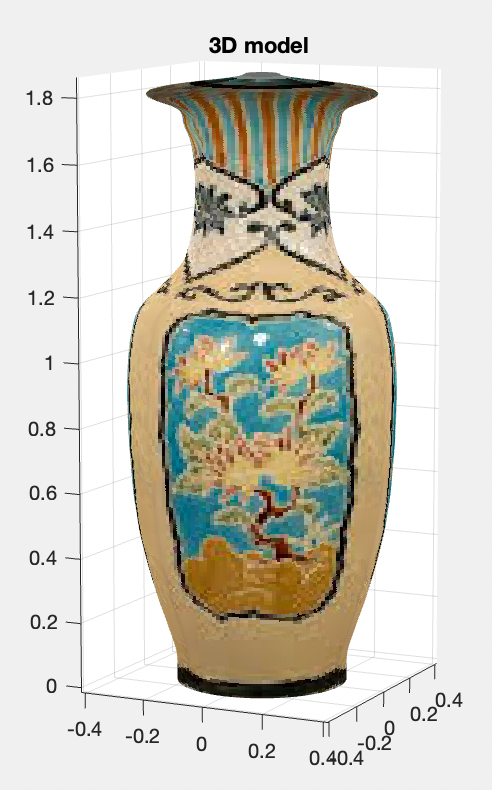
\includegraphics[height=5cm]{ourRes-14}\label{res3_3DOut:f1}}
	\qquad
	\subfloat[]{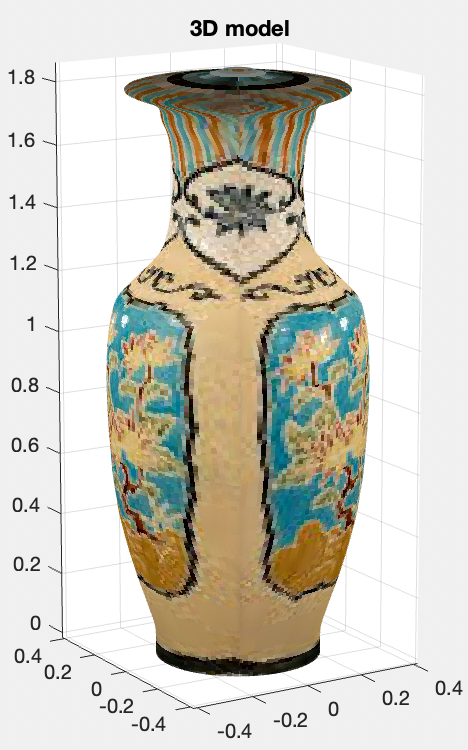
\includegraphics[height=5cm]{ourRes-15}\label{res3_3DOut:f2}}
	\caption{مدل سه‌بعدی بازسازی شده سوم}
	\label{res3_3DOut}
\end{figure}
\newline
ورودی بعدی اندکی با موارد قبلی تفاوت دارد. این ورودی (تصویر \ref{res4In:f1}) یک کوزه با تعداد تکرار‌های زیاد در الگوی تکرار شونده خود است. قطاع انتخاب‌شده در تصویر \ref{res4In:f2} آمده است. این قطاع نسبت به قطاع‌های قبلی باریک‌تر است اما برای بهتر دیده‌شدن، نسبت طول به عرض آن تغییر داده ‌شده است.
\begin{figure}[h!]
	\centering
	\subfloat[تصویر اصلی شیء]{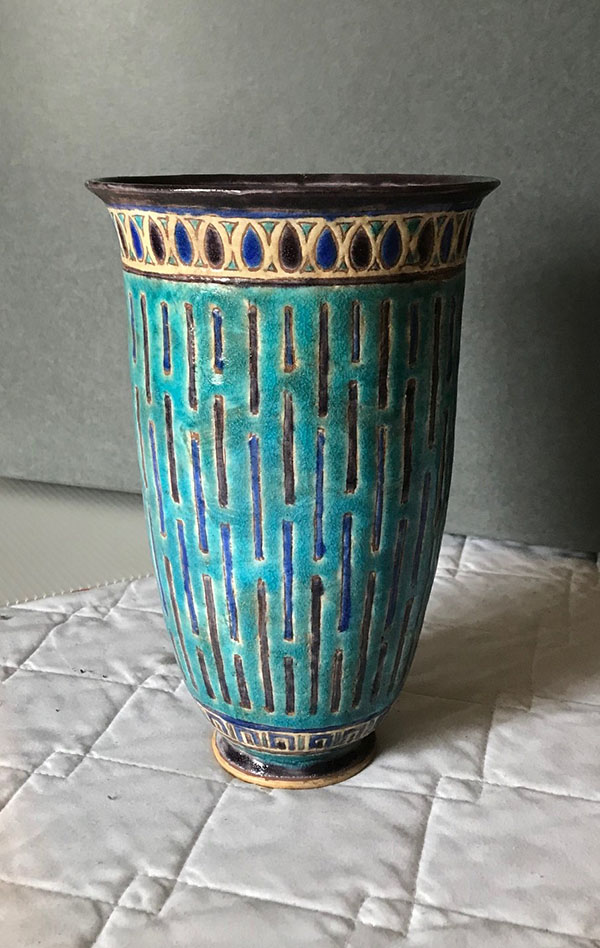
\includegraphics[height=4cm]{ourRes-16}\label{res4In:f1}}
	\qquad
	\subfloat[قطاع استخراج‌شده]{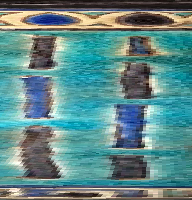
\includegraphics[height=4cm]{ourRes-17}\label{res4In:f2}}
	\caption{ورودی‌های چهارم الگوریتم ارائه‌شده}
	\label{res4In}
\end{figure}
\newline
بافت نهایی تولید‌شده برای این قطاع با شانزده تکرار در شکل \ref{res4Out} آمده است. این بافت به نظر هموار است و هم قسمت بالایی آن و هم قسمت پایینی آن به صورت مناسبی تکرار شده و به یکدیگر چسبانده شده است.
\begin{figure}[h!]
	\centering
	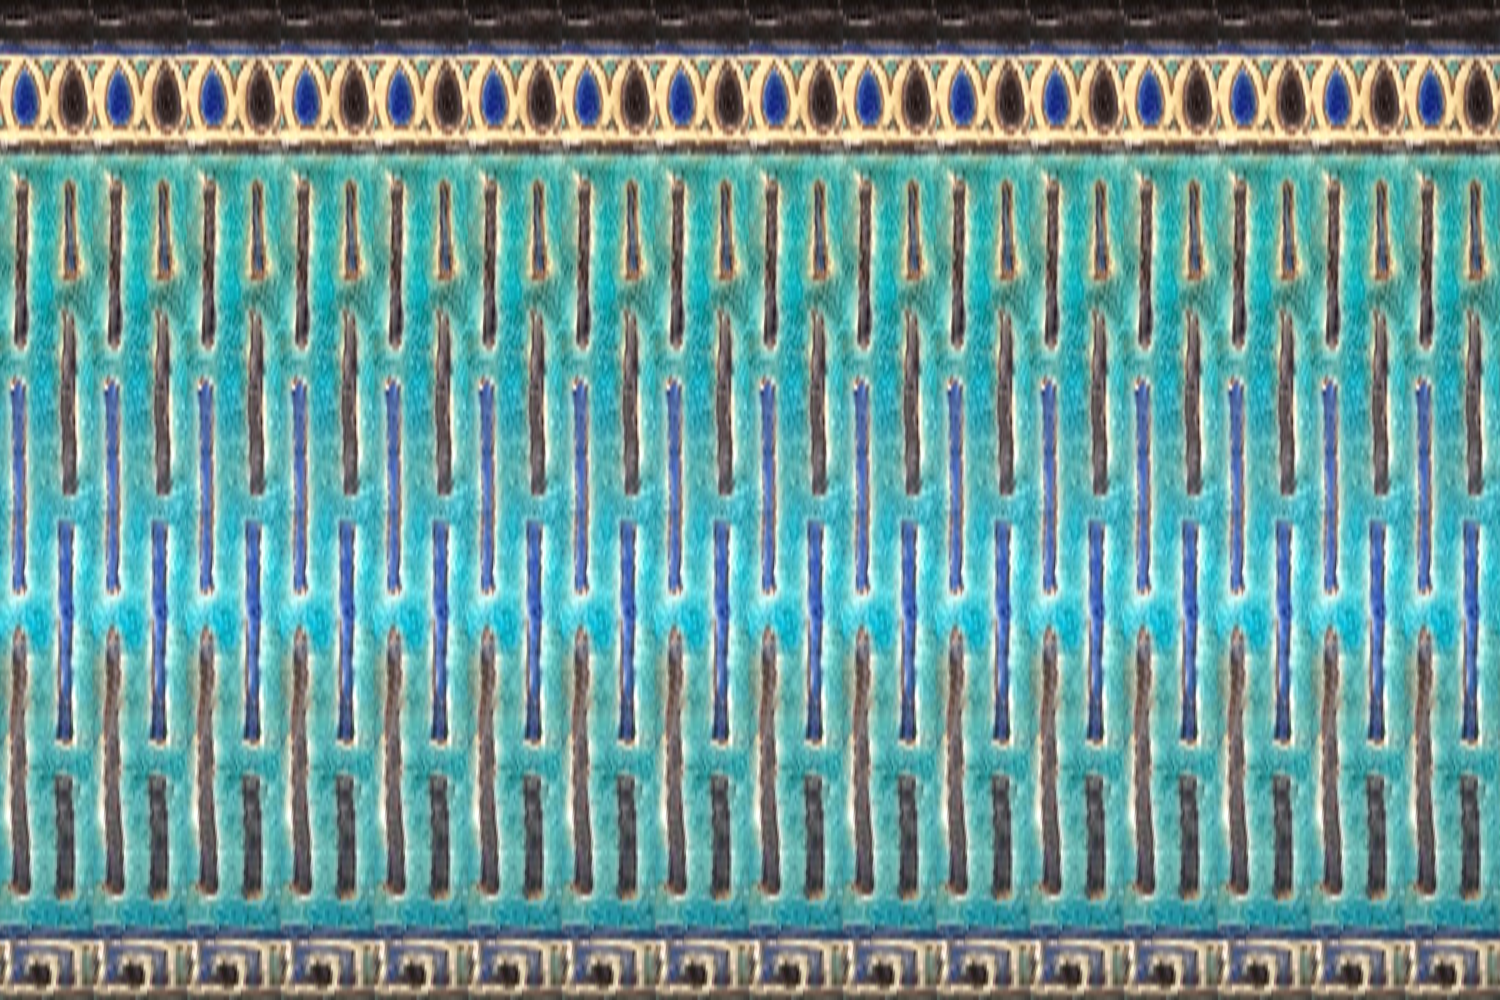
\includegraphics[height=5cm]{ourRes-18}
	\caption{بافت تولید شده از الگوریتم ارائه‌شده برای ورودی چهارم}
	\label{res4Out}
\end{figure}

در شکل \ref{res4_3DOut} مدل سه‌بعدی نهایی تولید‌شده مشخص است. این مدل از لحاظ ظاهری بسیار مشابه به شیء اصلی است و هم هندسه و هم بافت نهایی تولید شده مناسب بوده است.
\begin{figure}[h!]
	\centering
	\subfloat[]{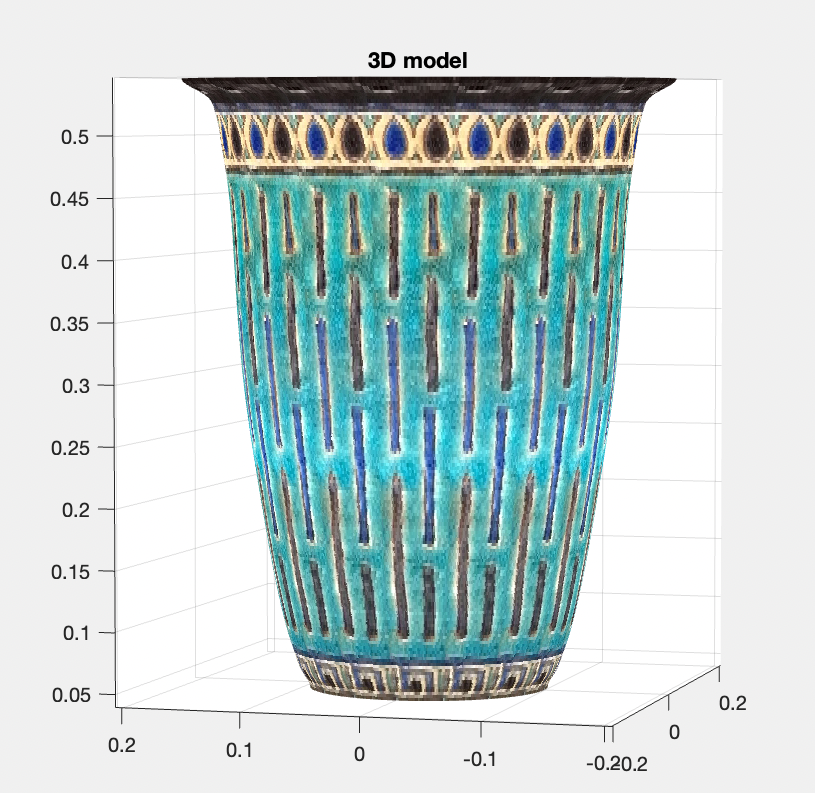
\includegraphics[height=5cm]{ourRes-19}\label{res4_3DOut:f1}}
	\qquad
	\subfloat[]{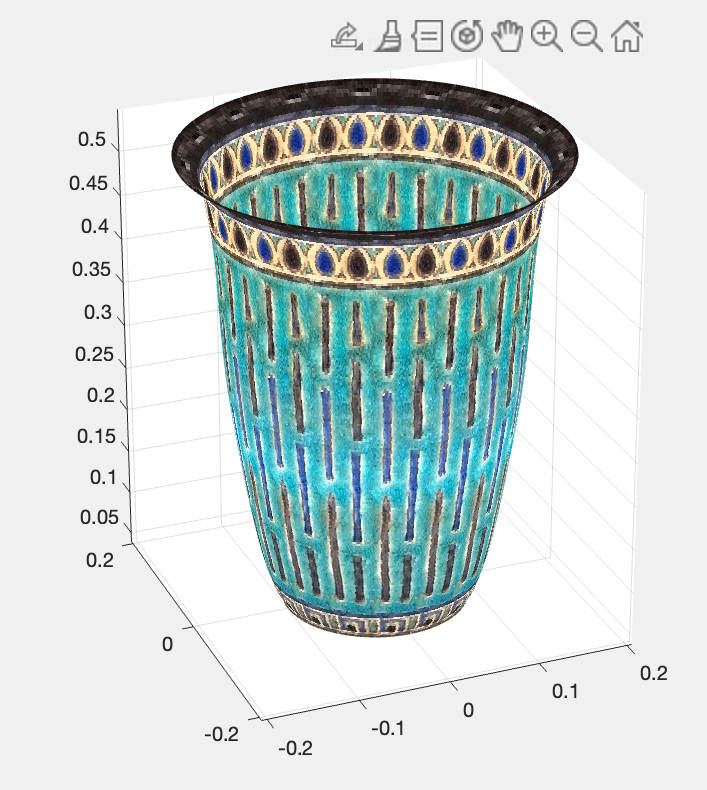
\includegraphics[height=5cm]{ourRes-20}\label{res4_3DOut:f2}}
	\caption{مدل سه‌بعدی بازسازی شده سوم}
	\label{res4_3DOut}
\end{figure}
\newline
در نمونه‌ی بعدی، شیء حاوی الگوی تکرارشونده‌ای نیست. این جسم (تصویر\ref{res5In:f1})، که یک بطری است، برای نمایش کاربرد الگوریتم ارائه‌شده در تکرار الگوی رویی برای قسمت پشت مدل سه‌بعدی آورده شده است. در شکل \ref{res5_bad} مدل سه‌بعدی بازسازی‌شده با استفاده از روش تکرار ساده الگوی رویی برای قسمت پشت آمده است. نتیجه‌ی این کار به نسبت مناسب است و مشکل زیادی ندارد. قطاع انتخاب شده برای الگوریتم ارائه‌شده در این حالت (تصویر \ref{res5In:f2}) همان الگوی رویی شیء در تصویر ورودی است که بدون بریدن به عنوان ورودی به الگوریتم ما داده می‌شود. 
\begin{figure}[h!]
	\centering
	\subfloat[تصویر اصلی شیء]{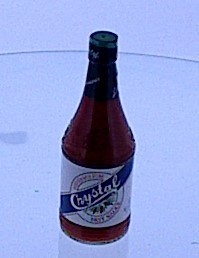
\includegraphics[height=4cm]{ourRes-21}\label{res5In:f1}}
	\qquad
	\subfloat[قطاع استخراج‌شده]{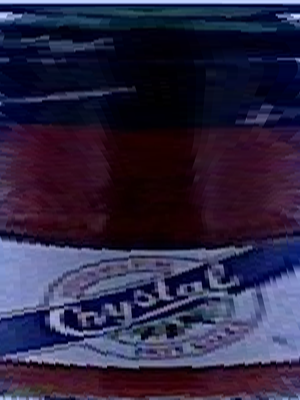
\includegraphics[height=4cm]{ourRes-22}\label{res5In:f2}}
	\caption{ورودی‌های پنجم الگوریتم ارائه‌شده}
	\label{res5In}
\end{figure}
\begin{figure}[h!]
	\centering
	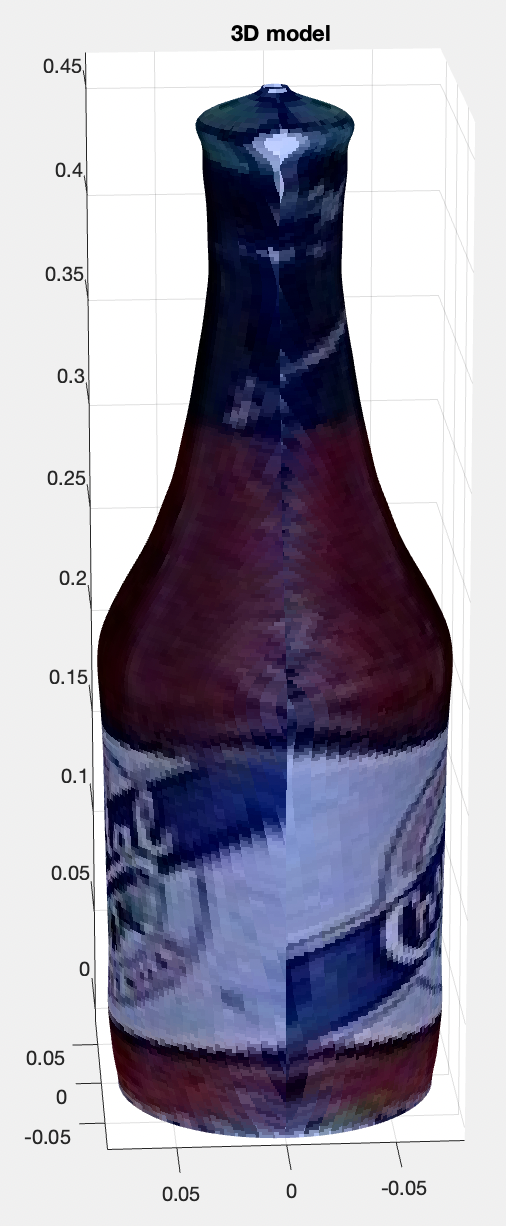
\includegraphics[height=5cm]{ourRes-26}
	\caption{مدل سه‌بعدی بازسازی‌شده برای ورودی پنجم با استفاده از تکرار ساده طرح رویی برای پشت}
	\label{res5_bad}
\end{figure}

بافت تولید شده در شکل \ref{res5Out} آمده است. همانطور که مشخص است، تعداد تکرار قطاع برای این بافت برابر دو بوده است. در خط میانی مشاهده می‌شود که خط جداکننده سنگینی وجود ندارد و به نسبت دو قطاع به صورت همواری به یکدیگر متصل شده‌اند. به خصوص در قسمت برچسب بطری، گذار از قسمت بنفش به رنگ پس‌زمینه‌ی برچسب هموارتر شده است و خط محکمی وجود ندارد.
\begin{figure}[h!]
	\centering
	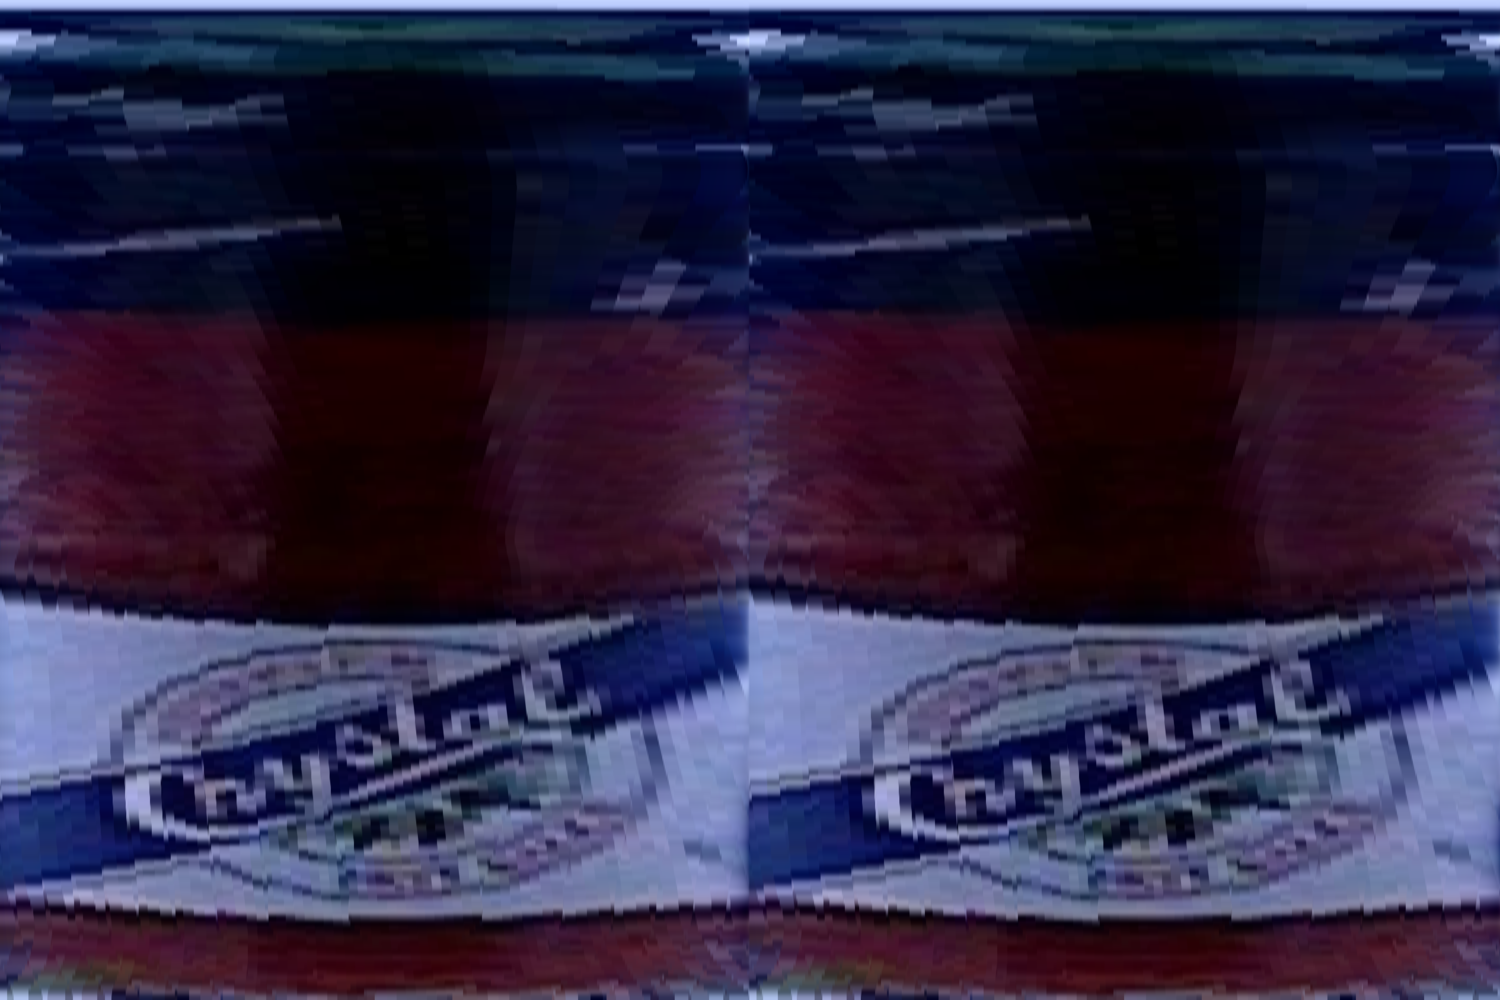
\includegraphics[height=5cm]{ourRes-23}
	\caption{بافت تولید شده از الگوریتم ارائه‌شده برای ورودی پنجم}
	\label{res5Out}
\end{figure}

شکل \ref{res5_3DOut} مدل سه‌بعدی بازسازی‌شده‌ی نهایی را در کنار مدل بازسازی شده با استفاده از روش تکرار ساده نمایش می‌دهد. همانطور که در مورد بافت تولید‌شده برای این شیء گفته‌شد، به نظر می‌آید با استفاده از الگوریتم ارائه‌شده، بافت اندکی هموارتر بوده و عملکردی تقریبا برابر با تکرار ساده بافت رویی برای قسمت پشت مدل سه‌بعدی داشته.
\begin{figure}[h!]
	\centering
	\subfloat[]{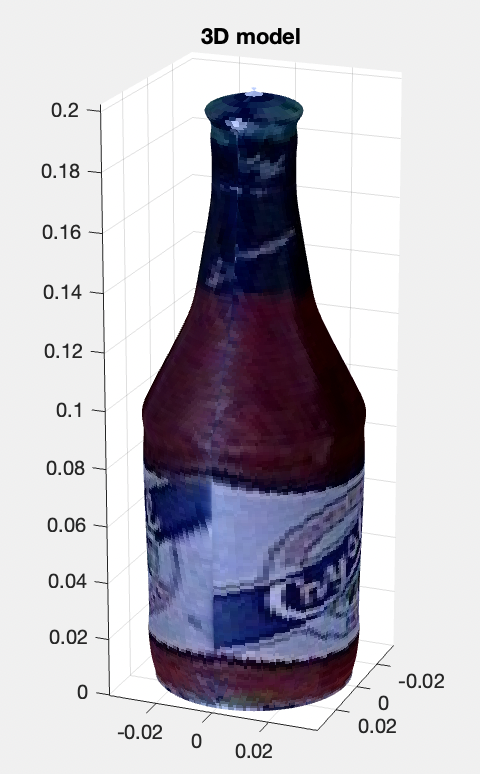
\includegraphics[height=5cm]{ourRes-24}\label{res5_3DOut:f1}}
	\qquad
	\subfloat[]{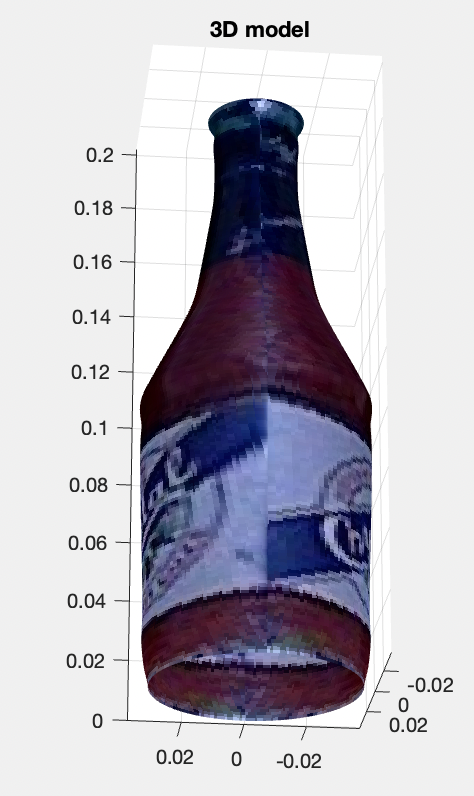
\includegraphics[height=5cm]{ourRes-25}\label{res5_3DOut:f2}}
	\caption{مدل سه‌بعدی بازسازی شده پنجم}
	\label{res5_3DOut}
\end{figure}

در انتها یک مثال آورده می‌شود که عملکرد الگوریتم ما مناسب نبوده است. شیء ورودی و قطاع استخراج‌شده از آن در شکل \ref{res6In} آمده است. همانطور که در تصویر قطاع مشخص است، قطاع طرح تکرارشونده را به صورت مناسب در بر گرفته، اما از سمت راست به چپ، در قسمت بالا‌ی قطاع، شدت نور در حال کاهش است و حاشیه‌ی سمت چپ قطاع با شروع سایه همراه بوده است. مشکل دیگری که دیده می‌شود، صاف نبودن خطوط پایینی الگو است که به علت مشکل در استخراج الگوی رویی پیش آمده. توانستیم با استفاده از روش رفع واپیچش خط‌های بالایی را صاف کنیم، اما خط‌های پایینی صاف نشدند.
\begin{figure}[h!]
	\centering
	\subfloat[تصویر اصلی شیء]{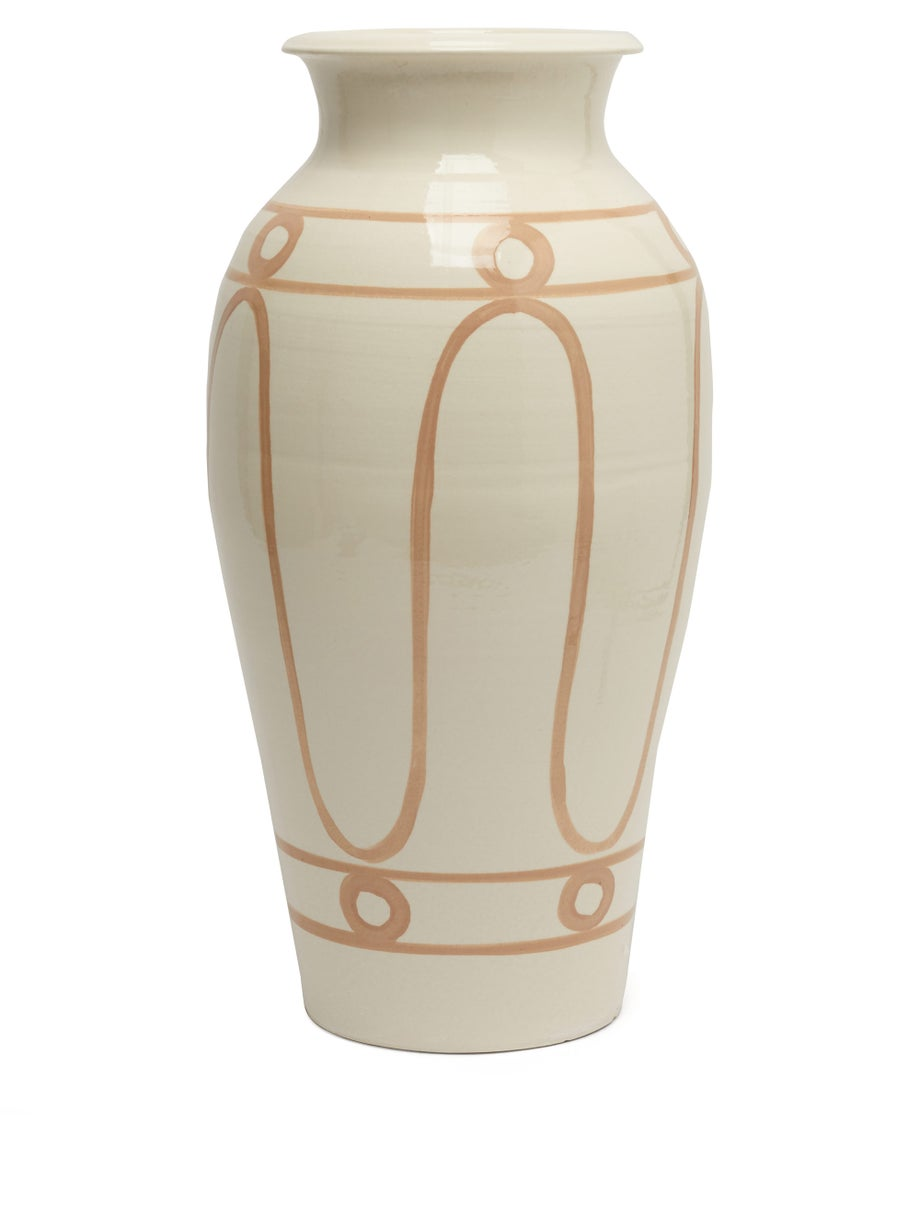
\includegraphics[height=4cm]{ourRes-27}\label{res6In:f1}}
	\qquad
	\subfloat[قطاع استخراج‌شده]{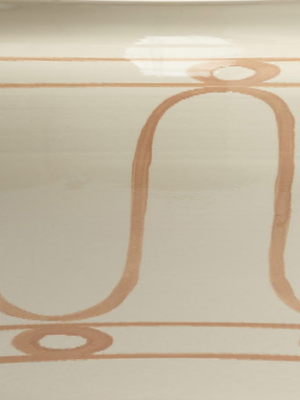
\includegraphics[height=4cm]{ourRes-28}\label{res6In:f2}}
	\caption{ورودی‌های ششم الگوریتم ارائه‌شده}
	\label{res6In}
\end{figure}

در شکل \ref{res6Out} بافت تولید شده برای این شیء آمده است. الگوریتم ما نتوانسته به صورت مناسب در قسمت بالا (به علت وجود سایه) و پایین (به علت صاف نبودن خطوط و وجود سایه) هموار کردن قطاع را انجام دهد. در قسمت میانی قطاع به علت صاف بودن و نبود سایه، هموار شدن به صورت مناسبی صورت گرفته است.
\begin{figure}[h!]
	\centering
	\includegraphics[height=5cm]{ourRes-30}
	\caption{بافت تولید شده از الگوریتم ارائه‌شده برای ورودی ششم}
	\label{res6Out}
\end{figure}

در تصویر \ref{res6_3DOut:f2} می‌توان مدل سه‌بعدی نهایی بعد از نگاشت بافت تولیدشده را دید. همانطور که در تصویر بافت هم دیدیم، مدل در قسمت بالا و پایین قطاع، ظاهر مناسبی ندارد و به صورت مناسب هموار نشده است. در تصویر \ref{res6_3DOut:f2} مدل نهایی تولید شده با استفاده از روش تکرار الگوی رویی برای پشتی آمده است که نشان می‌دهد عملکرد روش ما نسبت به این روش، بهتر بوده است.
\begin{figure}[h!]
	\centering
	\subfloat[روش تکرار]{\includegraphics[height=5cm]{ourRes-29}\label{res6_3DOut:f1}}
	\qquad
	\subfloat[الگوریتم ارائه‌شده]{\includegraphics[height=5cm]{ourRes-31}\label{res6_3DOut:f2}}
	\caption{مدل سه‌بعدی بازسازی شده ششم}
	\label{res6_3DOut}
\end{figure}

اولین علت این ضعف می‌تواند این موضوع باشد که الگوریتم ارائه‌شده تنها به حاشیه‌ها توجه می‌کند و نمی‌تواند ناسازگاری‌های الگو را در طول قطاع هموار کند. دومین علت نیز می‌تواند کم بودن مساحت در نظر گرفته شده برای ناحیه‌ی هم‌پوشانی باشد. با توجه به اینکه طول این ناحیه به صورت یک عدد ثابت در نظر گرفته شده، برای تصاویری که کیفیت بالاتر و تعداد پیکسل‌های بیشتری دارند، این مساحت می‌تواند به نسبت تعداد پیکسل‌های قطاع، کوچک باشد و باعث شود الگوریتم به درستی کار خود را انجام ندهد. در نظر گرفتن مساحت ناحیه‌ی هم‌پوشانی به صورت نسبتی از طول قطاع، امکان دارد نتایج را بهتر کند. البته باید دقت کرد این مساحت از تصویر ورودی الگو بیرون نزند. به طور مثال برای ورودی‌هایی که الگو برش‌ داده نمی‌شود، ناحیه‌ی هم‌پوشانی بزرگ می‌تواند نظم الگو را به هم بزند.

در انتها، جدول \ref{tab:timings} زمان اجرای روش ما برای ورودی‌های نمایش داده‌شده در این بخش را نمایش می‌دهد.
\newpage
\begin{table}[htbp]
	\caption{زمان اجرای الگوریتم}
	\label{tab:timings}
	\centering
	\onehalfspacing
	\begin{tabular}{ ||c c c c|| }
		\hline \rl{ورودی} & \rl{ابعاد قطاع} & \rl{تعداد تکرار قطاع} & \rl{مدت زمان (ثانیه)} \\ 
		\hline
		\hline \rl{ورودی اول \ref{res1In}} & \lr{$305*401$} & $12$ & $26.92$ \\ 
		\hline \rl{ورودی دوم \ref{res2In}} & \lr{$302*401$} & $8$ & $15.83$ \\ 
		\hline \rl{ورودی سوم \ref{res3In}} & \lr{$936*300$} & $3$ & $25.37$ \\ 
		\hline \rl{ورودی چهارم \ref{res4In}} & \lr{$192*200$} & $16$ & $5.61$ \\ 
		\hline \rl{ورودی پنجم \ref{res5In}} & \lr{$1270*200$} & $2$ & $12.09$ \\ 
		\hline \rl{ورودی ششم \ref{res6In}} & \lr{$476*500$} & $4$ & $24.59$ \\ 
		\hline
	\end{tabular}
\end{table}

